\documentclass[10pt,journal,compsoc]{IEEEtran}
\usepackage[T1]{fontenc}
\usepackage{cite}
\usepackage{amsmath,amssymb,amsfonts}
\usepackage{graphicx}
\usepackage{booktabs,tabularx,array}
\usepackage{xcolor}
\usepackage{tikz}
\usetikzlibrary{arrows.meta,positioning,fit}
\usepackage[hidelinks]{hyperref}
\usepackage{xurl}
\usepackage{subcaption}
\graphicspath{{figures/}}

\newcolumntype{Y}{>{\raggedright\arraybackslash}X}
\newcommand{\code}[1]{\texttt{\detokenize{#1}}}
\newcommand{\ind}{\mathbf{1}}
\newcommand{\reach}{\mathcal{D}}
\newcommand{\unknown}{\bot}
\definecolor{auditblue}{RGB}{26,67,107}
\definecolor{auditgold}{RGB}{168,102,24}
\interdisplaylinepenalty=2500
\newtheorem{proposition}{Proposition}
\newtheorem{theorem}{Theorem}

\newcommand{\PaperTitle}{Maintainer Prioritization in npm Supply Chains: Objectives, Representation Sensitivity, and Metadata Limits}

% Generated by scripts/render_research_figures.py from structural_interventions/results.json.
\newcommand{\StudyPackages}{25,228}
\newcommand{\StudyMaintainers}{12,217}
\newcommand{\StudyWorkflowPackages}{15,233}
\newcommand{\StudyWorkflowRepos}{7,171}
\newcommand{\GreedyCovered}{5,538}
\newcommand{\GreedyCoveragePercent}{77.2}
\newcommand{\GreedyExposurePercent}{11.48}
\newcommand{\UnionCovered}{4,407}
\newcommand{\UnionExposurePercent}{33.79}
\newcommand{\GreedyExcluded}{800}
\newcommand{\VersionPairsDecreasePercent}{42.44}
\newcommand{\ChangedRoots}{8,587}

% Generated rows: method, C count, C percent, H percent, P count; budget 100.
% Random row is the mean of 200 trials; figure random curve uses exact analytic expectation.
\newcommand{\ResearchMethodRows}{%
Portfolio & 4,579 & 63.9 & 7.96 & 577 \\%
Summed reach & 4,835 & 67.4 & 21.98 & 704 \\%
Maximum reach & 4,268 & 59.5 & 33.59 & 533 \\%
Exact union & 4,407 & 61.5 & 33.79 & 534 \\%
Greedy coverage & 5,538 & 77.2 & 11.48 & 800 \\%
Random (mean) & 1,680.6 & 23.4 & 0.80 & 12.8 \\%
}

% Generated from read-only workflow-repository reconciliation.
\newcommand{\QixPortfolio}{8}
\newcommand{\QixNameReach}{1,942}
\newcommand{\QixVersionReach}{1,476}
\newcommand{\QixUnionRank}{7}
\newcommand{\QixVersionRank}{5}
\newcommand{\QixHybridRank}{35}
\newcommand{\QixOutsideSindresorhus}{366}

% Generated revision evidence
\newcommand{\AuditSample}{120}
\newcommand{\AuditCommits}{115}
\newcommand{\HeuristicExactHits}{86}
\newcommand{\HeuristicExactSettings}{96}
\newcommand{\HeuristicWorstGap}{66}
\newcommand{\ReplicationEndpoints}{66}
\newcommand{\ReplicationAccounts}{1051}
\newcommand{\ReplicationPairDecrease}{3.33}
\newcommand{\ReplicationGreedyC}{65}
\newcommand{\ReplicationUnionC}{42}

\newcommand{\ArtifactAccessStatement}{The October graph-validation data, analysis tables, protocols and checksums are in a versioned public archive. The named version supplies the release link and fixed original-input reference. Third-party workflow and manifest bodies are referenced by pinned source URLs and hashes.}

\begin{document}

\title{\PaperTitle}

\author{Anonymous authors}

\markboth{Maintainer Prioritization in npm Supply Chains}%
{Maintainer Prioritization in npm Supply Chains}

\IEEEtitleabstractindextext{%
\begin{abstract}
\textbf{Context.} Teams that can review only a fixed number of npm maintainer accounts need to know which downstream applications those accounts cover.

\textbf{Objective.} We ask whether preserving dependency paths across exact package versions changes which applications a fixed-size selection covers.

\textbf{Method.} Before gathering consumer evidence, we select five accounts using each of two npm graph representations. In two held-out application catalogs, we trace paths in committed lockfiles and use registry records for the locked versions to check for selected accounts. We count confirmed changes in coverage and use the unresolved cases to bound turnover, the share of applications reached by exactly one selection.

\textbf{Results.} The YunoHost comparison confirms five switches. The name portfolio alone reaches three applications and the version portfolio alone reaches two. With follow-up checks, 164 of 215 pairs are resolved and turnover lies between 2.3\% and 26.0\%. In Awesome-Selfhosted, 88 of 155 pairs are resolved, with no confirmed switches and turnover bounded at 0--43.2\%. The net direction remains unresolved in both frames. An exploratory YunoHost check finds a separate switch at 50 accounts. On the original graph at budget 100, greedy coverage reaches 5,538 repositories and exact union reaches 4,407, with modeled exposure reductions of 11.48\% and 33.79\%, respectively.

\textbf{Conclusion.} At a fixed account budget, keeping track of which applications enter or leave review scope reveals changes that a net coverage count can miss.
\end{abstract}

\begin{IEEEkeywords}
Software supply chain security, npm ecosystem, maintainer prioritization, multi-objective optimization, dependency graphs, release authority.
\end{IEEEkeywords}}

\maketitle
\IEEEdisplaynontitleabstractindextext
\IEEEpeerreviewmaketitle

\section{Introduction}
\IEEEPARstart{N}{pm} dependency and maintainer relations can concentrate downstream reach in a small set of accounts. Zimmermann et al. examined npm maintainer influence, combined reach and vetting.\footnote{Zimmermann et al., \emph{Small World with High Risks}, USENIX Security 2019. \url{https://www.usenix.org/conference/usenixsecurity19/presentation/zimmerman}} A review program must also specify what a limited account budget should accomplish. Reaching many distinct repositories, removing account-origin exposure, and selecting every observed source are different objectives.

Consider two accounts whose portfolios reach many of the same repositories. After selecting the first, the second may add little distinct coverage while remaining a possible origin in a structural exposure model. An endpoint can therefore be covered while retaining many unselected sources. Mathematical definitions establish that these quantities differ; an empirical study must measure how consequential the distinction is and how observation choices affect the comparison.

We compare the objectives on a retained, high-impact-seeded npm graph containing 25,228 identifiers, including bundled contexts, and 12,217 observed usernames. The main endpoint universe contains 7,171 normalized workflow-associated repository keys. These units are neither a registry-wide sample nor observations of installed-code execution. We evaluate established ranking and greedy-coverage baselines~\cite{nemhauser1978}, exploratory scalarization, and an exclusion-oriented heuristic.

We assess the comparison through component benchmarks, a new acquisition and an automated endpoint-evidence audit. Component ablations and small exact benchmarks test whether the exclusion heuristic's additional scoring is useful. A new acquisition from 100 frozen, sampled roots tests transport to a bounded cohort with fresh dependency, maintainer and workflow observations. A stratified probability sample of 120 endpoints supplies commit-pinned evidence about repository mappings and workflow files. Automated indicators characterize this evidence; their accuracy was not manually validated.

We ask four questions:
\begin{itemize}
\item \textbf{RQ1:} How large are the observed coverage, additive-exposure and all-source-exclusion tradeoffs at equal budgets?
\item \textbf{RQ2:} How do representation choices affect evaluation, and what evidence supports the workflow-associated endpoint observations?
\item \textbf{RQ3:} How sensitive is the exclusion-oriented heuristic to its components, candidate cap and ties, and where does it miss candidate-restricted optima?
\item \textbf{RQ4:} Which tradeoffs persist in a new bounded acquisition and a common-population comparison?
\end{itemize}

Our contribution is measured evidence about these decision and observation choices. The additive optimum and standard submodular guarantee supply the theoretical foundations. The simpler exclusion heuristic slightly improves exclusion on the original graph but underperforms the original heuristic in the new cohort. The additional acquisition repeats the coverage--exposure tradeoff while substantially changing the size of representation effects. A separate application pilot measures the feasibility of tracing selections through committed consumer dependencies. Two held-out frames measure which consumers have documented paths to distinct five-account portfolios and quantify the uncertainty from unresolved evidence.

\section{Related Work}
\label{sec:related_work}

\subsection{Upstream Prioritization}
Schueller and Wachs model how developer departures and failure propagation jointly affect Rust libraries, then compare allocations of developer support~\cite{schueller2024}. Hamer et al. combine contributor network measures with survey evidence to study contributor reputation in dependency review~\cite{hamer2025trust}. In npm, Samaana et al. find that dependency depth affects measured technical leverage~\cite{samaana2025}. He et al. use simulated dependency resolution to study local pinning and coordinated changes at selected upstream packages~\cite{he2025}. We hold the account budget fixed, compare coverage and exclusion objectives, and evaluate whether representation changes which consumers have documented paths to selected accounts.

\subsection{Consumer and Release Evidence}
Zerouali et al. examine release gaps, maintainer activities, and outdated dependencies in dormant npm packages~\cite{zerouali2026dormant}. Mohayeji et al. measure developers' responses to Dependabot security updates~\cite{mohayeji2025}. Jayasuriya et al. examine breaking changes associated with transitive dependencies~\cite{jayasuriya2024}. These studies motivate retaining dependency versions and observation dates. Our outcome concerns a documented dependency path at a pinned commit. Developer response and adoption require separate observations.

Bifolco et al. measure discrepancies in GitHub dependency and dependent records for Java and Python projects~\cite{bifolco2025accuracy}. Wang et al. characterize resolution across ten package managers and reconstruct registry dependencies over time with OpenDep~\cite{wang2026opendep}. Gamage et al. compare lockfile design and maintenance across seven package managers~\cite{gamage2026lockfiles}. Our paired analysis joins registry account associations to version-resolved paths from a specified application importer.

Bi et al. document recurring challenges from SBOM generation through consumption~\cite{bi2024sboms}. Xiao et al. find dependency omissions in developer-published Java SBOMs~\cite{xiao2025sbom}. This motivates checking the exact recipe asset, the metadata's subject, and the dependency information it contains. A source revision can support a comparison of declared dependencies. Evidence of bundled components requires inspecting the delivered artifact or an inventory linked to its bytes.

Table~\ref{tab:lit_positioning} compares the closest empirical studies and their observation units.

\begin{table*}[t]
\centering
\small
\caption{Closest empirical work and the additional question addressed here. Different observation units prevent direct comparison of reported security percentages.}
\label{tab:lit_positioning}
\begin{tabularx}{\textwidth}{lYYYY}
\toprule
Study & Population & Main observations & Validation basis & Additional question here\\
\midrule
\cite{schueller2024} & Rust ecosystem & Risks shared across developers and libraries & Modeled developer departure and dependency failures & Account selections under different dependency representations\\
\cite{samaana2025} & npm library releases & Technical leverage & Replication across dependency depths & Sensitivity of fixed-budget selection\\
\cite{he2025} & npm projects and registry & Local pinning and coordinated version constraints & Historical resolution simulations & Account selection evaluated against committed consumer paths\\
\cite{wang2026opendep} & Ten package managers & Ecosystem-scale dependency resolution & Policy characterization and resolution checks & Importer and artifact evidence for paired application outcomes\\
This study & Retained graph, bounded training cohort and separate application frame & Objective tradeoffs and reassignment under equal budgets & Pinned consumer paths and independently collected registry records & Projects uniquely reached by either selection and limits from unresolved evidence\\
\bottomrule
\end{tabularx}
\end{table*}

\section{Data Corpus and Graph Construction}
\label{sec:data_construction}
\subsection{Collection and Units}
The collector starts with high-impact npm packages and expands their dependency graphs through deps.dev\footnote{\url{https://docs.deps.dev/api/v3/}}. It requests registry metadata and checks linked repositories for a \code{.github/workflows} directory at GitHub HEAD. Queue dates span June 13--16, 2026. Individual fields lack a common acquisition cutoff. The archive analyzed on October 20 contains 25,228 graph identifiers, 22,340 version-metadata rows, 12,217 maintainer usernames, and 79,405 package--maintainer relations. Registry membership records observed associations at collection time.

Among these identifiers, 2,745 encode bundled contexts rather than independently registered packages. The 121,885 retained version-edge rows project to 88,113 distinct name adjacencies. Stored \code{DIRECT}/\code{INDIRECT} labels describe a target node relative to an extraction root; their 48,705/73,180 row counts do not partition global direct and transitive edges. We reverse every explicit declaring-to-dependency adjacency to measure downstream reach.

Figure~\ref{fig:q1_observation_workflow} summarizes the collection and analysis architecture.

\begin{figure*}[t]
\centering
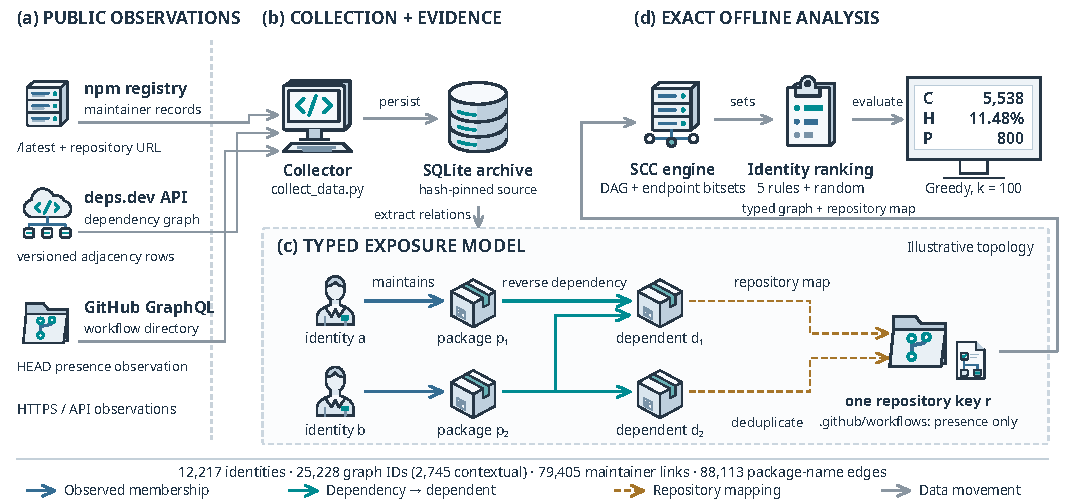
\includegraphics[width=0.96\textwidth]{study_system.pdf}
\caption{Measurement architecture: (a) public observations, (b) collection and retained evidence, (c) typed exposure model, and (d) offline analysis. Icons denote logical roles and topology is illustrative. Counts and displayed greedy outcomes are empirical; workflow presence does not establish execution.}
\label{fig:q1_observation_workflow}
\end{figure*}

The 15,233 package names with a positive workflow-directory observation map to 7,171 repository keys. We case-fold owner and repository names and remove trailing \code{.git} using lexical rules. The archive has 3,081 identifiers without maintainer mappings and 3,772 without completed workflow flags. A zero flag can mean directory absence or repository unavailability. Coverage uses all 7,171 repository endpoints with a positive observation. Exclusion counts use the 7,158 endpoints with an observed source.

\begin{figure*}[t]
\centering
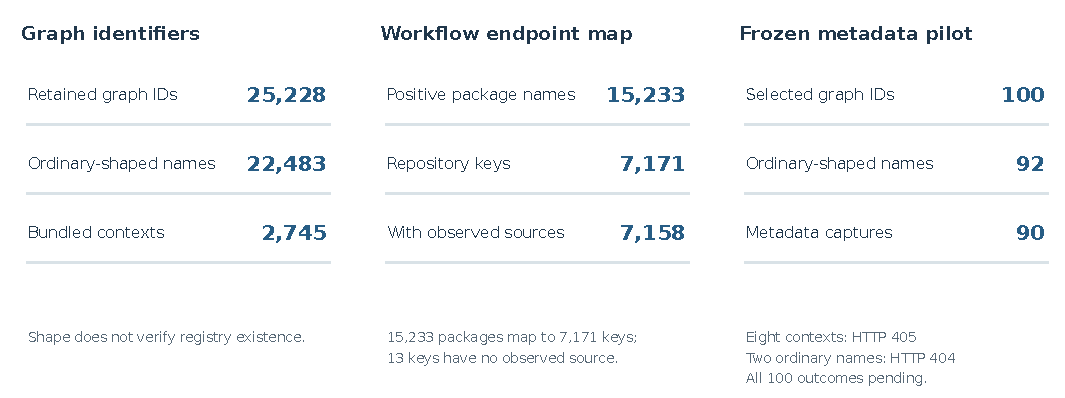
\includegraphics[width=0.94\textwidth]{observation_scope.pdf}
\caption{Observation units and metadata acquisition. Panels describe separate populations; their missingness counts must not be added across panels. Context identifiers are retained graph units, not separate registry packages. The metadata pilot sampled 100 identifiers before requests; its observed request outcomes are shown separately.}
\label{fig:q1_observation_scope}
\end{figure*}

Figure~\ref{fig:q1_observation_scope} separates graph units, observed workflow endpoints, and the metadata-pilot sampling frame. This distinction matters because directory observation and metadata acquisition do not validate a historical installation or a future outcome.

\subsection{Name Projection and Exact-Version Continuity}
The name graph merges retained versions sharing an identifier. The sensitivity graph retains 40,806 exact (package, version) nodes and joins paths only at matching version keys. A maintained package seeds every retained version; without a version node, it contributes only its eligible seed endpoint. Both representations use the same package-level workflow flags. Neither reproduces npm installation or historical lockfile behavior: contexts and acquisition times remain mixed.

\subsection{Automated Endpoint Evidence Audit}
Before new audit requests, we freeze 120 endpoints drawn without replacement from the 7,158 repositories with observed sources. Four source-count strata contain 1,716 endpoints with one source, 1,473 with two to five, 1,959 with six to fifty, and 2,010 with more than fifty; each contributes 30 sampled repositories. Inclusion probabilities and design weights are retained. Failed observations are not replaced. Equal stratum allocation means the unweighted pooled support percentage is not an estimate for the full frame.

For each endpoint, acquisition requests its original package/version registry metadata, resolves a repository commit, and retrieves workflow files, candidate package manifests and root lockfiles at that commit. It records response states, timestamps, commit IDs and file hashes. Up to twenty workflow files and twelve manifest/lockfile candidates per repository are retained under the frozen request limits. Mapping support requires matching evidence for every package/version observation assigned to the endpoint; monorepo paths and unresolved reusable actions can leave labels unknown.

The automated pass records 172 version-specific registry-request outcomes and 115 pinned repository commits. It flags 106 endpoints as mapping-support candidates, 115 with workflow files, 88 with aligned installation directives, 70 with root lockfiles, and 17 with dependency/version examples. Table~\ref{tab:revision_audit} and Figure~\ref{fig:revision_audit_benchmarks}(a) describe these machine-generated evidence candidates. These indicators were not manually validated and are not estimates of historical mapping precision.
% Generated by scripts/render_journal_validation.py
\begin{table*}[t]
\centering
\footnotesize
\caption{Automated evidence candidates in the frozen 120-endpoint audit. Labels await independent author review.}
\label{tab:revision_audit}
\begin{tabular}{lrr}
\toprule
Evidence criterion & Candidate support & Unresolved\\
\midrule
All package mappings supported & 106 & 14\\
Workflow file acquired & 115 & 5\\
Aligned install directive & 88 & 32\\
Relevant root lockfile & 70 & 50\\
Dependency/version example & 17 & 103\\
\bottomrule
\end{tabular}
\par\smallskip\begin{minipage}{0.98\textwidth}\footnotesize The 115 acquired commits are current-time observations. Unresolved states are not negative or safe outcomes; candidate support is not human-validated precision. All mappings assigned to an endpoint must match for the first criterion.\end{minipage}
\end{table*}


\begin{figure*}[t]
\centering
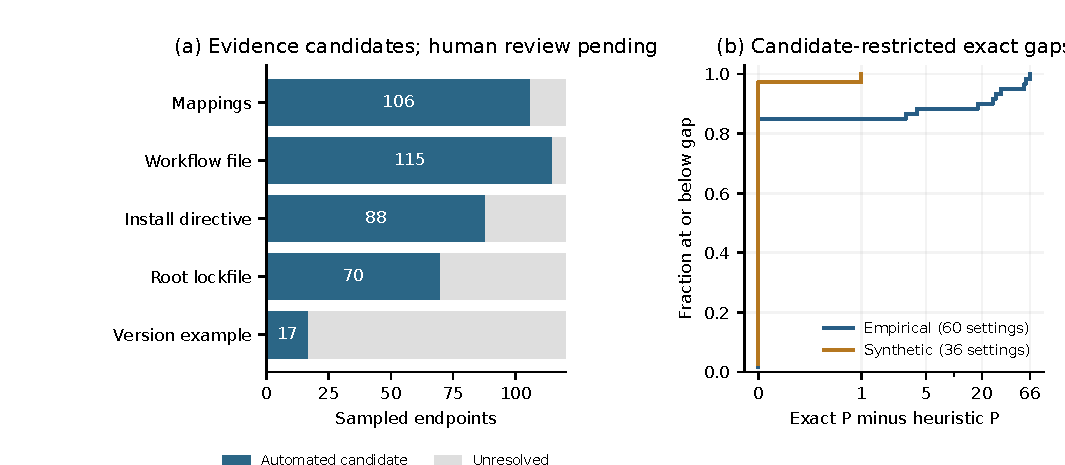
\includegraphics[width=0.98\textwidth]{revision_audit_benchmarks.pdf}
\caption{Evidence diagnostics: (a) automatically extracted endpoint indicators and unresolved cases; (b) empirical and synthetic candidate-restricted exact exclusion gaps. Panel populations and inferential meanings differ. The exact settings reuse instances across budgets.}
\label{fig:revision_audit_benchmarks}
\end{figure*}

Current-commit evidence cannot retrospectively validate the original undated HEAD observations. Static installation commands do not establish executed jobs, and a lockfile example does not validate every transitive path. Frozen original account selections are evaluated on progressively stricter machine-evidence subsets as provisional diagnostics in the replication materials. Full source sets are preserved. Design-weighted C/P totals and H pair-mass ratios are distinguished from conditional subset results; unresolved-included/excluded H scenarios are not claimed as sharp bounds.

Figure~\ref{fig:q1_version_semantics} illustrates how version merging can introduce a path absent from the exact-version graph.

\begin{figure}[t]
\centering
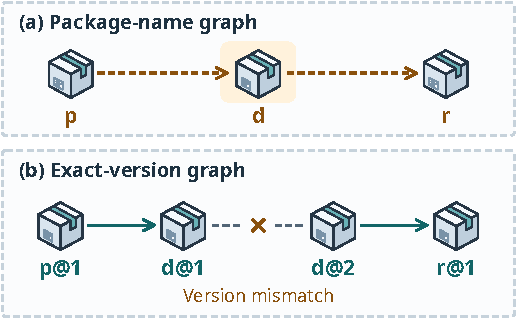
\includegraphics[width=\columnwidth]{graph_semantics.pdf}
\caption{Illustrative version splicing. The name graph merges d@1 and d@2 into d, creating apparent reach from p to r. Dashed amber arrows show projected reverse reach. Solid teal arrows show the two exact-version paths.}
\label{fig:q1_version_semantics}
\end{figure}

\subsection{Cycles, Mapping Disagreements and Contexts}
The name graph has 82 nontrivial strongly connected components (SCCs) containing 403 nodes; the exact-version union has 68 containing 304 nodes. The largest component has 61 nodes in each. SCC condensation preserves reach and permits exact bitset propagation over a directed acyclic graph; the implementation uses arbitrary-precision Python integers, not fixed 64-bit sets. This is a computation technique, not an intervention that removes cycles.

The URL audit finds 658 identifier-level parser disagreements. Excluding 60 inconsistent positive observations reduces the workflow repository universe to 7,147; greedy at budget 100 gives $C=5{,}524$ and $P=799$. We discard ambiguous flags rather than transferring them to a corrected URL without reacquisition. Removing bundled-context nodes preserves all 462,170 primary account--repository incidences for fixed selections, although workflow-package incidence changes. That invariance does not apply automatically to every endpoint definition or individual-package ranking.

OpenAI Codex assisted with development and checking of the analysis scripts. The scripts apply the stated extraction and scoring rules directly to the retained inputs. Recomputing the reported outcomes uses the scripts and captured records without calling a language model. Figures were generated with Matplotlib and editable vector artwork. Numerical plot data are included in the replication artifact.

\section{Objectives and Optimization Framework}
\label{sec:objectives}

Let $S$ be the set of accounts selected for review. Its size is the account budget. The original graph has $|M|=12{,}217$ accounts and $|R_{\text{wf}}|=7{,}171$ workflow-associated repository keys. For each account $m\in M$, $E_m\subseteq R_{\text{wf}}$ contains the repositories reachable from packages associated with $m$. For repository $r$, $\operatorname{Sources}(r)=\{m\in M:r\in E_m\}$ is its set of observed upstream sources.

Figure~\ref{fig:q1_methodology} summarizes the analysis and consistency checks.

\begin{figure}[t]
\centering
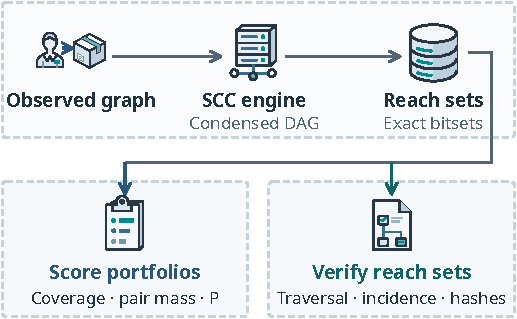
\includegraphics[width=\columnwidth]{study_methodology.pdf}
\caption{The observed graph yields exact reach sets through strongly connected component condensation and bitset unions. The sets supply both fixed-budget scoring and reachability checks. Comparisons use the same graph within each representation.}
\label{fig:q1_methodology}
\end{figure}

\subsection{Graph Objectives}

\subsubsection{Submodular Distinct Coverage ($C(S)$)}
Distinct coverage counts each reachable repository once.
\begin{equation}
C(S) = \Bigl\lvert \bigcup_{m \in S} E_m \Bigr\rvert .
\end{equation}
$C(\varnothing)=0$, and coverage is monotone and submodular. For $A\subseteq B\subseteq M$ and $m\notin B$,
\begin{equation}
C(A \cup \{m\}) - C(A) \ge C(B \cup \{m\}) - C(B)
\end{equation}
The classical Nemhauser--Wolsey--Fisher bound gives greedy coverage a $(1-1/e)\approx63.2\%$ approximation. For a normalized, monotone submodular objective $F$ and budget $k\ge1$, let $O$ be an optimal set. The sum of the marginal gains of $O\setminus S_i$ at the current greedy set $S_i$ is at least $F(O)-F(S_i)$. Greedy therefore removes at least $1/k$ of the remaining gap each step. After $k$ steps, the achieved value is at least $[1-(1-1/k)^k]F(O)\ge(1-1/e)F(O)$.

\subsubsection{Modular Scenario Exposure Reduction ($H(S)$)}
Assign each hypothetical origin $m$ a fixed nonnegative weight $w_m$. Under ideal selected-origin removal, all $|E_m|$ account--repository pairs from a selected origin are removed. When total weighted pair mass is positive, its removed share is
\begin{equation}
H(S) = \frac{\sum_{m \in S} w_m |E_m|}{\sum_{v \in M} w_v |E_v|}
\end{equation}
$H(\varnothing)=0$, and $H$ is monotone and modular. For disjoint $A$ and $B$, $H(A\cup B)=H(A)+H(B)$. Sorting in descending order of $w_m|E_m|$ therefore maximizes $H$ at each budget. We call this rule exact union. Unit weights give the unweighted pair-mass comparison.

\subsubsection{Supermodular All-Source Exclusion ($P(S)$)}
Under the same idealized model, an endpoint has no remaining observed source when every member of its nonempty source set is selected:
\begin{equation}
P(S) = \sum_{r \in R_{\text{wf}}}
  \ind\bigl[\varnothing \ne \operatorname{Sources}(r) \subseteq S\bigr].
\end{equation}
\textbf{Property:} $P(S)$ is \textit{supermodular}. Selecting maintainer $m$ contributes zero gain to $r$ until its final unselected source is selected. For $A\subseteq B$ and $m\notin B$,
\begin{equation}
P(A \cup \{m\}) - P(A) \le P(B \cup \{m\}) - P(B).
\end{equation}

\subsubsection{Strict Zero-Anchored Threshold Exclusion ($P_k$)}
Let $n_r=\lvert\operatorname{Sources}(r)\rvert$ and
$t_r(S)=\lvert\operatorname{Sources}(r)\setminus S\rvert$. In this definition, the positive integer threshold $k$ is independent of the budget $|S|$. For $R_+=\{r\in R_{\text{wf}}\mid n_r>0\}$,
\begin{equation}
\begin{aligned}
P_k(S) &= \sum_{r\in R_+} \ind\bigl[t_r(S)<q_k(r)\bigr],\\
q_k(r) &=
  \begin{cases}
    1, & n_r<k,\\
    k, & n_r\ge k .
  \end{cases}
\end{aligned}
\label{eq:strict_quorum}
\end{equation}
For $n_r<k$, the rule credits complete source exclusion. For $n_r\ge k$, it credits fewer than $k$ remaining sources. Thus $P_k(\varnothing)=0$, $P_1(S)=P(S)$, and every counted endpoint has a selected source. The count is monotone in $S$ for a fixed threshold. An endpoint with $n_r=2$ and $t_r(S)=1$ qualifies at $k=2$ and ceases to qualify at $k=3$, so counts can decrease as the threshold increases.

The cardinality guard removes zero-budget credit but does not supply missing authorization semantics. It is an explicit modeling convention, not evidence that a repository actually implements a $k$-person approval policy; upstream source sets may span independently compromised packages.

\subsection{Proposition 1: Monotone Submodularity of Hybrid Scalarization $J_\alpha(S)$}
To examine choices between coverage and conditional exposure, we evaluate the standard scalarization:
\begin{equation}
J_\alpha(S) = \alpha \cdot \frac{C(S)}{|R_{\text{wf}}|} + (1 - \alpha) \cdot H(S)
\end{equation}
where $\alpha \in [0, 1]$ parameterizes defensive posture between broad coverage ($\alpha = 1$) and scenario exposure reduction ($\alpha = 0$).

\begin{proposition}
For any $\alpha \in [0, 1]$, the objective $J_\alpha(S)$ is monotone non-decreasing and submodular.
\end{proposition}
\begin{IEEEproof}
Let $A \subseteq B \subseteq M$ and $m \notin B$. The marginal gain is:
\begin{equation}
\begin{aligned}
\Delta J_\alpha(m \mid S)
  &= \alpha \frac{\bigl\lvert E_m \setminus \bigcup_{u\in S} E_u\bigr\rvert}
                  {\lvert R_{\text{wf}}\rvert} \\
  &\quad + (1-\alpha)\frac{w_m\lvert E_m\rvert}
                           {\sum_{v\in M} w_v\lvert E_v\rvert} .
\end{aligned}
\end{equation}
The second term is constant with respect to $S$ (modular), so its marginal difference across $A$ and $B$ is exactly zero. The first term satisfies submodularity by set-theoretic inclusion:
\begin{equation}
|E_m \setminus \bigcup_{u \in A} E_u| \ge |E_m \setminus \bigcup_{u \in B} E_u|
\end{equation}
The sum of a submodular function and a modular function is submodular, so $J_\alpha$ is submodular for all $\alpha\in[0,1]$. Lazy evaluation preserves the greedy marginal choice. The gap argument for $C$ therefore also gives the $(1-1/e)$ guarantee for $J_\alpha$.
\end{IEEEproof}

\subsection{Supermodular Minimum-Remaining-Source Heuristic for $P(S)$}
Because $P(S)$ is supermodular, greedy coverage and exact union achieve all-source exclusion purely as an unoptimized side-effect. To directly optimize $P(S)$, we design an adaptive minimum-remaining-source heuristic. At each step, let $\text{rem}(r)=\text{Sources}(r)\setminus S$. Candidate maintainers are drawn from endpoints with one to ten remaining sources; if none exist, all unselected maintainers are considered. The implementation maximizes a lexicographic tuple: (i) the number of endpoints immediately completed, (ii) the sum of $1/|\text{rem}(r)|$ over affected endpoints with more than one remaining source, (iii) marginal coverage, and (iv) ascending maintainer index. This is a heuristic with no global optimality guarantee for $P(S)$.

\subsection{Heterogeneous Maintainer Risk Formulations}
We evaluate three structural models of non-uniform maintainer risk:
\begin{enumerate}
    \item \textbf{Single-Maintainer Bottlenecks ($w_m^{\text{sole}}$):} Packages with $|M(p)|=1$ have one observed maintainer; actual review practices are unobserved. We weight maintainers by $w_m^{\text{sole}} = 1 + |\{p \in P_m : |M(p)| = 1\}|$.
    \item \textbf{Log-Portfolio Activity ($w_m^{\text{log}}$):} As an assumed portfolio-size sensitivity, define: $w_m^{\text{log}} = 1 + \log_2(1 + |P_m|)$.
    \item \textbf{Package-Level Sole-Maintainer Reach ($H_{\text{pkg-sole}}$):} Instead of weighting all reachable repositories of maintainer $m$, we isolate repositories reachable strictly through $m$'s sole-maintained packages: $E_m^{\text{sole}} = \bigcup_{p \in P_m, |M(p)|=1} \reach(p)$.
\end{enumerate}

\subsection{Analytic Expectations and Empirical Standard Errors}
A uniform sample of $k$ accounts without replacement gives each account inclusion probability $k/|M|$. This yields the expected exposure by linearity. The expected coverage uses the hypergeometric probability of selecting at least one source per repository.
\begin{align}
\mathbb{E}[H_{\text{rand}}(k)] &= \frac{k}{\lvert M\rvert}, \\
\mathbb{E}[C_{\text{rand}}(k)] &= \sum_{r \in R_{\text{wf}}}
  \left( 1 - \frac{\binom{\lvert M\rvert-n_r}{k}}
                  {\binom{\lvert M\rvert}{k}} \right).
\end{align}
For $k = 100$, exact finite-population expectations are $\mathbb{E}[C] = 1{,}716.8$ and $\mathbb{E}[H] = 0.819\%$. Across 200 simulation seeds, the sample mean coverage is 1,680.6 (sample standard deviation $\text{SD}_C = 530.7$, Monte Carlo Standard Error $\text{MCSE}_C = 37.5$), and sample mean exposure reduction is $0.80\%$ ($\text{SD}_H = 0.373\text{ pp}$, $\text{MCSE}_H = 0.026\text{ pp}$). Replicated offline execution across 3 independent runs averaged $39.50\text{ s}$ wall-clock time with $1{,}038.43\text{ MiB}$ peak RSS.

\subsection{Use of AI Assistance}
OpenAI Codex was used to assist with manuscript drafting, revision, and checking literature sources. The authors are responsible for the manuscript, its interpretation, and its references.

\section{Core Tradeoffs and Representation: RQ1 and RQ2}
\label{sec:empirical_results}

We first compare the objectives across account budgets on the original graph. We then examine how overlapping sources and exact package versions affect those comparisons.

Figure~\ref{fig:q1_source_partition} partitions covered endpoints by whether any unselected source remains.

\begin{figure}[t]
\centering
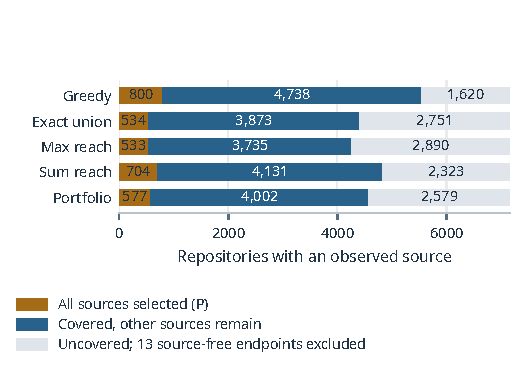
\includegraphics[width=\columnwidth]{coverage_partition.pdf}
\caption{Budget-100 repository partition. Each bar separates all-source exclusion, coverage with residual sources, and uncovered endpoints. The 13 source-free endpoints are omitted. Structural coverage and complete exclusion differ for every baseline.}
\label{fig:q1_source_partition}
\end{figure}

\subsection{RQ1: Coverage vs. Additive Exposure Trade-Off}
Figure~\ref{fig:objective_tradeoff} shows how coverage and exposure vary with budget. Table~\ref{tab:multi_budget_comparison} reports outcomes at $|S|\in\{1,5,10,25,50,100\}$. Selecting 100 accounts uses $0.819\%$ of the 12,217 observed accounts.

% Generated by scripts/reconcile_full_manuscript.py
\begin{table*}[t]
\centering
\footnotesize
\caption{Workflow-repository outcomes from the retained baseline experiment. Random entries are 200-order sample means and Monte Carlo standard errors, not population confidence intervals.}
\label{tab:multi_budget_comparison}
\begin{tabular}{llrrrrrr}
\toprule
Budget & Metric & Portfolio & Sum & Max & Exact union & Greedy & Random mean $\pm$ MCSE\\
\midrule
1 & C (\%) & 23.43 & 33.02 & 28.75 & 35.46 & 35.46 & 0.65 $\pm$ 0.19\\
1 & H (\%) & 0.36 & 0.51 & 0.45 & 0.55 & 0.55 & 0.01 $\pm$ 0.00\\
1 & P & 1 & 26 & 2 & 269 & 269 & 0.28 $\pm$ 0.15\\
5 & C (\%) & 46.00 & 49.25 & 42.14 & 50.96 & 54.00 & 2.61 $\pm$ 0.36\\
5 & H (\%) & 1.16 & 2.15 & 2.23 & 2.45 & 2.09 & 0.04 $\pm$ 0.01\\
5 & P & 316 & 325 & 80 & 329 & 327 & 0.69 $\pm$ 0.17\\
10 & C (\%) & 47.90 & 51.75 & 42.81 & 54.53 & 60.40 & 4.73 $\pm$ 0.46\\
10 & H (\%) & 1.59 & 2.68 & 4.06 & 4.48 & 3.79 & 0.08 $\pm$ 0.01\\
10 & P & 391 & 399 & 111 & 343 & 351 & 1.21 $\pm$ 0.19\\
25 & C (\%) & 56.71 & 60.95 & 45.29 & 59.74 & 67.69 & 10.15 $\pm$ 0.55\\
25 & H (\%) & 4.38 & 7.45 & 9.00 & 9.86 & 6.08 & 0.21 $\pm$ 0.01\\
25 & P & 430 & 480 & 116 & 427 & 514 & 2.86 $\pm$ 0.26\\
50 & C (\%) & 62.00 & 63.78 & 45.56 & 60.26 & 72.46 & 16.73 $\pm$ 0.56\\
50 & H (\%) & 6.14 & 13.72 & 17.19 & 18.09 & 8.73 & 0.43 $\pm$ 0.02\\
50 & P & 503 & 576 & 117 & 441 & 638 & 5.97 $\pm$ 0.38\\
100 & C (\%) & 63.85 & 67.42 & 59.52 & 61.46 & 77.23 & 23.44 $\pm$ 0.52\\
100 & H (\%) & 7.96 & 21.98 & 33.59 & 33.79 & 11.48 & 0.80 $\pm$ 0.03\\
100 & P & 577 & 704 & 533 & 534 & 800 & 12.78 $\pm$ 1.42\\
\bottomrule
\end{tabular}
\end{table*}



\begin{figure*}[t]
\centering
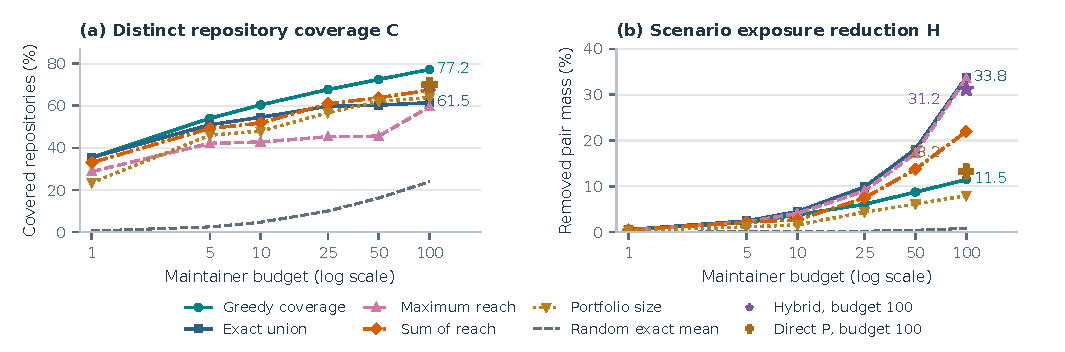
\includegraphics[width=0.92\textwidth]{objective_tradeoff.pdf}
\caption{Multi-budget trade-off trajectories across maintainer budgets $|S| \in [1, 100]$: (a) submodular coverage $C(S)$, (b) modular scenario exposure reduction $H(S)$, using five deterministic rules and the exact random expectation. Budget-100 markers show hybrid and direct-exclusion selections.}
\label{fig:objective_tradeoff}
\end{figure*}

At budget 100, greedy coverage reaches 5,538 repositories (77.23\%) and exact union reaches 4,407 (61.46\%). The difference is 1,131 repositories, or 15.77 percentage points. Exact union attains $H=33.79\%$ and greedy coverage attains $H=11.48\%$. The exposure difference from unrounded values is 22.30 percentage points.

Exact union's H advantage follows from its additive objective under equal costs. The experiment measures the accompanying loss in distinct coverage. Greedy offers the largest measured coverage among the compared baseline selections; it is an approximation to maximum coverage, not a proved global optimum. Portfolio size gives 63.85\% coverage and 7.96\% H at this budget, showing that portfolio count and measured downstream reach need not agree.

\subsection{Residual Sources and Single-Source Fragility}
A repository can have many source accounts even when a single account already covers it. Across the 7,158 repositories with observed sources, mean source cardinality is 64.57 and the maximum is 1,502. These are graph source identities, not measured permissions or independent compromises. Figure~\ref{fig:q1_source_distribution} shows their distribution and the remaining-source distributions after budget-100 selections.

\begin{figure*}[t]
\centering
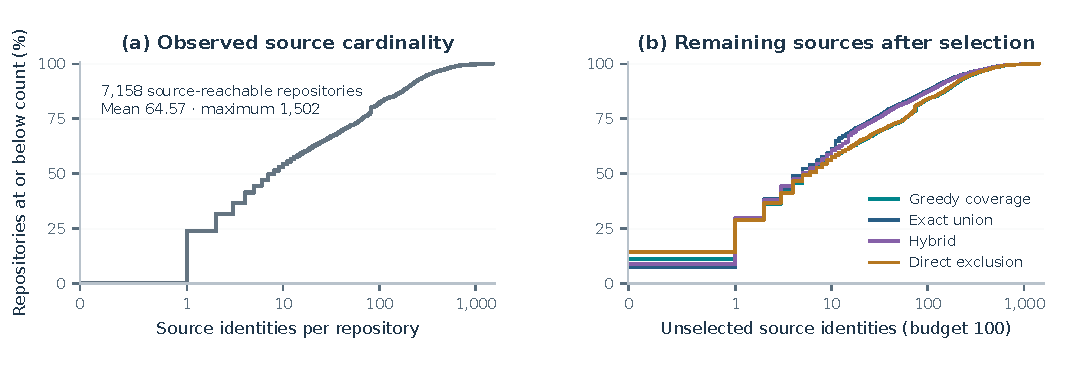
\includegraphics[width=0.94\textwidth]{source_multiplicity.pdf}
\caption{Observed source multiplicity and residual-source distributions at budget 100. All curves use the same 7,158 source-reachable repositories; 13 source-free endpoints are excluded. Zero remaining sources identify all-source exclusions. Horizontal scales are logarithmic above one. Account origins are structural scenarios, not observed compromises.}
\label{fig:q1_source_distribution}
\end{figure*}

Greedy's $P=800$ is 11.18\% of source-reachable repositories; exact union gives $P=534$. Consequently, 6,358 source-reachable repositories retain at least one unselected source after greedy selection. A four-source illustration would retain three source identities when one is selected, but that fraction is not an estimated compromise probability.

\begin{figure}[t]
\centering
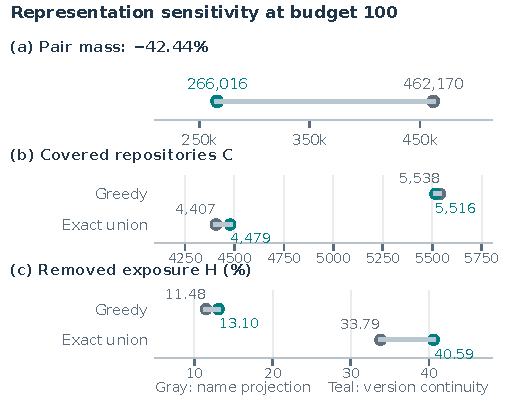
\includegraphics[width=\columnwidth]{representation_detail.pdf}
\caption{Cross-representation divergence: preserving exact-version continuity removes some paths introduced by version merging and reduces total identity-repository exposure pairs by $42.44\%$, shifting maintainer leverage. Gray denotes name projection and teal denotes version continuity.}
\label{fig:representation_detail}
\end{figure}

\subsection{RQ2: Version-Continuity Representation and Selection Penalties}
Figure~\ref{fig:representation_detail} summarizes pair mass and budget-100 outcomes under the two representations.
Comparing the package-projected name graph against the observed exact-version edge union reveals substantial sensitivity to representation:
\begin{enumerate}
    \item \textbf{Exposure Shrinkage:} Preserving version continuity contracts total maintainer-repository exposure pairs from $462{,}170$ to $266{,}016$---an exact reduction of \textbf{$42.44\%$}.
    \item \textbf{Root Scope Changes:} $8{,}587$ out of $25{,}228$ graph identifiers ($34.04\%$) exhibit divergent downstream reach scopes between name-collapsed and version-continuous representations.
    \item \textbf{Cycle Condensation:} Kosaraju condensation detects $403$ nodes in $82$ nontrivial strongly connected components in the name graph, compared to $68$ cyclic components across $40{,}806$ version nodes in the version-continuous graph.
    \item \textbf{Version-Splicing Witnesses:} Retained representation diagnostics include five illustrative roots whose name-level paths lack a continuous counterpart in the retained version graph: \texttt{pseudomap}, \texttt{is}, \texttt{foreach}, \texttt{indexof}, and \texttt{has-color}.
\end{enumerate}

\subsubsection{The Cross-Representation Selection Penalty}
For the \texttt{sum\_package\_reach} heuristic at budget 100, the version-based ranking covers $34.34\%$ of version-based exposure. The name-based ranking covers $20.91\%$ on that same evaluation graph. Evaluating both selections on the version graph gives a difference of 13.43 percentage points.

\subsubsection{Cross-Sectional Incident-Associated Illustrations}
Table~\ref{tab:q1_incident_case_study} details reach metrics and maintainer prioritization ranks across the 16 incident-associated records whose package names occur in the retained graph.

% Generated by scripts/reconcile_full_manuscript.py
\begin{table*}[t]
\centering
\footnotesize
\caption{Observed workflow-repository reach and account rankings for 16 incident-associated records (15 package names). Reach and ranks use the retained cross-sectional graph, not pre-event installations.}
\label{tab:q1_incident_case_study}
\begin{tabularx}{\linewidth}{@{}Ylrrrrrr@{}}
\toprule
Package / record & Account (count) & Name reach & Version reach & Portfolio & Greedy & Union & Hybrid\\
\midrule
\texttt{debug} & \texttt{qix} (2) & 1,462 & 1,162 & \#2,298 & \#>100 & \#7 & \#35\\
\texttt{chalk} & \texttt{sindresorhus} (1) & 1,125 & 587 & \#2 & \#1 & \#1 & \#1\\
\texttt{ansi-styles} & \texttt{sindresorhus} (1) & 1,376 & 740 & \#2 & \#1 & \#1 & \#1\\
\texttt{simple-swizzle} & \texttt{qix} (1) & 120 & 31 & \#2,298 & \#>100 & \#7 & \#35\\
\texttt{backslash} & \texttt{qix} (1) & 0 & 0 & \#2,298 & \#>100 & \#7 & \#35\\
\texttt{eslint-config-prettier} & \texttt{lydell} (3) & 10 & 10 & \#561 & \#41 & \#102 & \#31\\
\texttt{eslint-plugin-prettier} & \texttt{lydell} (6) & 5 & 5 & \#561 & \#41 & \#102 & \#31\\
\texttt{@solana/web3.js} & \texttt{solana-devs} (1) & 4 & 4 & \#181 & \#>100 & \#1,752 & \#465\\
\texttt{nx} & \texttt{jameshenry} (8) & 2 & 2 & \#31 & \#>100 & \#835 & \#1,171\\
\texttt{node-ipc (v12)} & \texttt{riaevangelist} (12) & 4 & 4 & \#2,562 & \#>100 & \#3,163 & \#1,274\\
\texttt{node-ipc (v10)} & \texttt{riaevangelist} (12) & 4 & 4 & \#2,562 & \#>100 & \#3,163 & \#1,274\\
\texttt{@tanstack/history} & \texttt{tannerlinsley} (5) & 1 & 1 & \#163 & \#>100 & \#1,423 & \#455\\
\texttt{@ctrl/tinycolor} & \texttt{scttcper} (1) & 10 & 9 & \#5,765 & \#>100 & \#2,333 & \#1,227\\
\texttt{@opensearch-project/opensearch} & \texttt{peterzhuamazon} (3) & 0 & 0 & \#2,548 & \#>100 & \#1,491 & \#2,323\\
\texttt{@mastra/core} & \texttt{tylerbarnes} (9) & 0 & 0 & \#416 & \#>100 & \#6,314 & \#6,697\\
\texttt{echarts-for-react} & \texttt{atool} (1) & 0 & 0 & \#398 & \#>100 & \#1,945 & \#747\\
\bottomrule
\end{tabularx}
\par\smallskip\begin{minipage}{0.98\textwidth}\footnotesize Every account rank uses workflow-associated repository endpoints. The parenthesized value counts observed maintainers of that package. Membership is not evidence of historical publishing authority. Version labels and dependency counts are retained in the companion CSV. Package reach excludes the root; account portfolios include eligible seeds.\end{minipage}
\end{table*}


The individual-package comparison shows representation-dependent reach: \texttt{simple-swizzle} has 120 name-projected and 31 exact-version-continuous workflow endpoints; \texttt{chalk} has 1,125 and 587; \texttt{ansi-styles} has 1,376 and 740; \texttt{debug} has 1,462 and 1,162. These differences do not prove which paths an actual installation could execute.

The account-level example uses the same workflow endpoint definition. \texttt{qix} reaches \QixNameReach{} workflow repositories and ranks \#\QixUnionRank{} by exact union; version continuity yields \QixVersionReach{} and rank \#\QixVersionRank{}. It is beyond greedy's first 100 selections, while the hybrid places it \#\QixHybridRank{}. This illustrates overlap in current retained memberships, not a successful pre-event forecast or historical publisher attribution.

\begin{figure*}[t]
\centering
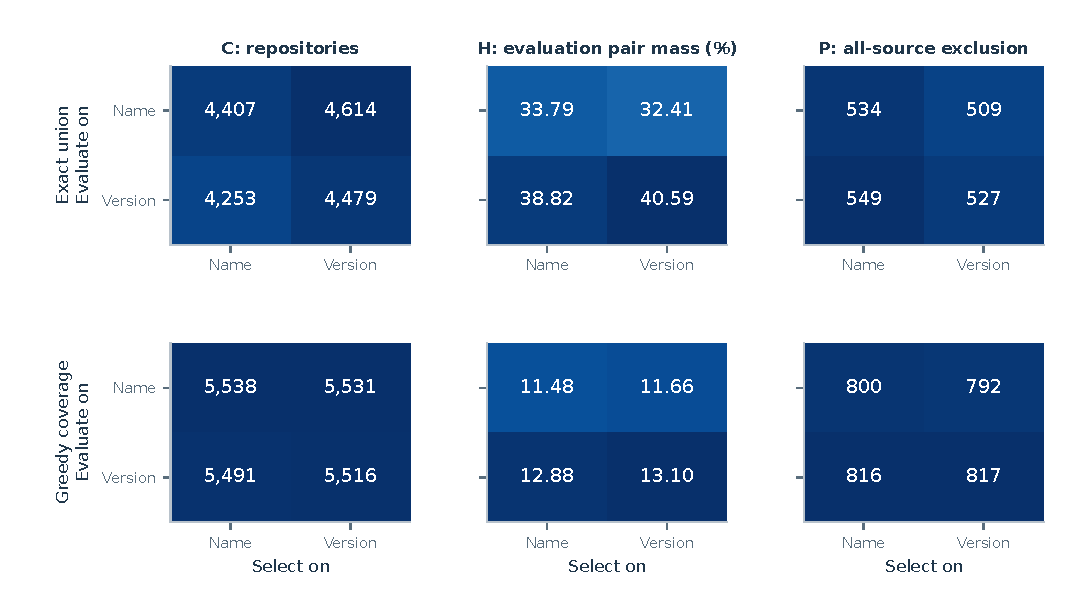
\includegraphics[width=0.98\textwidth]{representation_matrix.pdf}
\caption{Budget-100 selection/evaluation combinations for exact union and greedy. C and P count workflow repositories; H is divided by all account--repository pairs in the evaluation representation (462,170 for names; 266,016 for versions). Panels are separate metrics, not a common color scale.}
\label{fig:q1_representation_matrix}
\end{figure*}

Figure~\ref{fig:q1_representation_matrix} separates the representation used for selection from the one used for evaluation. Comparisons of H within an evaluation row share a denominator; comparisons across rows change that denominator. A change in representation can therefore change both the selection and the quantity being measured.

\section{Exclusion Heuristic Validation: RQ3}
\label{sec:pareto_and_weights}
\subsection{Baseline Gain and Component Ablations}
On the original graph, the direct heuristic yields $P=1{,}022$ at budget 100, compared with greedy coverage's 800 and exact union's 534. The same selection covers 5,020 distinct endpoints and reduces modeled exposure by 13.23\%. Table~\ref{tab:q1_supermodular_p} and Figure~\ref{fig:q1_supermodular_p_weights} report the multi-budget comparison.
% Auto-generated Supermodular P(S) Optimization Table for Q1 Journal Expansion
\begin{table*}[t]
\centering
\small
\caption{All-source exclusion $P(S)$ optimization via greedy minimum-source heuristic versus baseline single-objective rankings.}
\label{tab:q1_supermodular_p}
\begin{tabular}{rrrrrrrr}
\toprule
Budget & \multicolumn{3}{c}{Direct $P(S)$ Heuristic} & Greedy $P$ & Union $P$ & Gain vs Gr. & Gain vs Un.\\
\cmidrule(lr){2-4}
$|S|$ & $P$ & $C$ (\%) & $H$ (\%) & & & $\Delta P$ & $\Delta P$\\
\midrule
10 & \textbf{479} & 55.4\% & 2.58\% & 351 & 343 & +128 & +136\\
25 & \textbf{618} & 59.1\% & 4.15\% & 514 & 427 & +104 & +191\\
50 & \textbf{803} & 64.2\% & 6.55\% & 638 & 441 & +165 & +362\\
100 & \textbf{1,022} & 70.0\% & 13.23\% & 800 & 534 & +222 & +488\\
\bottomrule
\end{tabular}
\end{table*}


\begin{figure}[t]
\centering
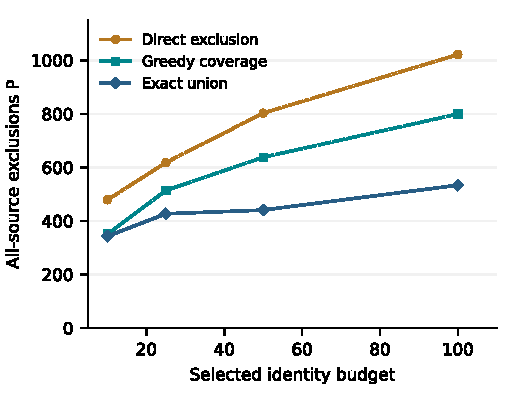
\includegraphics[width=\columnwidth]{q1_supermodular_p.pdf}
\caption{All-source exclusion under the original heuristic and coverage/exposure baselines. Counts describe the retained graph under ideal selected-source hardening.}
\label{fig:q1_supermodular_p_weights}
\end{figure}

The ablation analysis parameterizes the original lexicographic rule and reproduces its complete retained 100-account order before introducing variants. It changes the candidate cap to 1, 5, 20 and unrestricted, removes reciprocal remaining-source scoring or the coverage tie-break, and repeats tied choices under 30 frozen seeds. These are component sensitivities, not independent ecosystem observations.
% Generated by scripts/render_journal_validation.py
\begin{table*}[t]
\centering
\footnotesize
\caption{Budget-100 component ablations on the original graph. Timing is one selection run in the same process.}
\label{tab:revision_heuristic}
\begin{tabular}{lrrrr}
\toprule
Rule & $C$ & $H$ (\%) & $P$ & Seconds\\
\midrule
Original rule (cap 10) & 5,020 & 13.23 & 1,022 & 19.56\\
Immediate + coverage & 5,043 & 11.75 & 1,024 & 13.65\\
No coverage tie-break & 5,020 & 13.23 & 1,022 & 13.64\\
Cap 1 & 5,020 & 13.23 & 1,022 & 4.96\\
Cap 5 & 5,020 & 13.23 & 1,022 & 11.45\\
Cap 20 & 5,020 & 13.23 & 1,022 & 17.63\\
No candidate cap & 5,020 & 13.23 & 1,022 & 89.10\\
\bottomrule
\end{tabular}
\par\smallskip\begin{minipage}{0.98\textwidth}\footnotesize Immediate + coverage omits reciprocal remaining-source scoring and is identical to the no-reciprocal variant. Thirty seeded tie runs each give $P=1{,}022$ at budget 100; this is selection variability on one graph, not ecosystem uncertainty.\end{minipage}
\end{table*}


Removing reciprocal scoring gives $P=1{,}024$, two more than the original rule, together with $C=5{,}043$ and $H=11.75\%$. The immediate-completion variant uses coverage then identity order to resolve zero-gain cases. Candidate-cap changes and removing the coverage tie-break retain the original budget-100 P on this graph. All 30 tie runs also yield $P=1{,}022$. These outcomes provide no evidence that the reciprocal term improves original-graph exclusion; its usefulness must be assessed across other observed populations. Single-run timing in Table~\ref{tab:revision_heuristic} characterizes the implementation rather than a hardware-independent performance guarantee.

\subsection{Candidate-Restricted Exact Benchmarks}
We freeze 20 empirical candidate pools and 12 synthetic overlap instances, each with 20 eligible accounts and budgets 1, 3 and 5. Exhaustive enumeration evaluates every eligible subset. Empirical instances preserve complete endpoint source sets: sources outside the candidate pool remain unselected and can prevent exclusion. Candidate pools are constructed from low-cardinality source sets and reach-ranked fill accounts, so these are tractable diagnostic instances rather than a random sample of full-graph optimization problems.
Table~\ref{tab:revision_exact} reports the restricted-optimum comparisons.
% Generated by scripts/render_journal_validation.py
\begin{table*}[t]
\centering
\footnotesize
\caption{Exact exclusion benchmarks with 20 eligible accounts and budgets 1, 3 and 5.}
\label{tab:revision_exact}
\begin{tabular}{lrrrr}
\toprule
Instance family & Settings & Exact hits & Worst gap & Min ratio (\%)\\
\midrule
Empirical candidate pools & 60 & 51 & 66 & 16.46\\
Synthetic overlap instances & 36 & 35 & 1 & 93.33\\
\bottomrule
\end{tabular}
\par\smallskip\begin{minipage}{0.98\textwidth}\footnotesize Twenty empirical pools and twelve synthetic instances each supply three correlated budget settings. Outside-candidate sources remain unselected. Optima apply only to the restricted instance; no full-graph approximation guarantee follows.\end{minipage}
\end{table*}


The original heuristic reaches the restricted optimum in \HeuristicExactHits{} of \HeuristicExactSettings{} settings. It matches 51 of 60 empirical settings and 35 of 36 synthetic settings. Its worst empirical deficit is \HeuristicWorstGap{} endpoints and its minimum achieved-to-optimal ratio is 16.46\%; the worst synthetic deficit is one endpoint. Figure~\ref{fig:revision_audit_benchmarks}(b) shows the gap distributions. The 96 settings reuse 32 instances across budgets and are not independent replicates. These diagnostics identify substantive failure cases; neither the hit count nor the synthetic results certify the original full graph's optimum or an approximation ratio.

\subsection{Other Objective Choices}
Standard scalarization exposes intermediate coverage--exposure choices, but a preferred weight requires review costs and stakeholder preferences that were not measured. Additional heterogeneous weights, strict thresholds and uniform-efficacy multipliers are reported in Appendix~\ref{sec:objective_supplement}. A threshold sensitivity is not a count of empirically protected repositories: source identities are not authenticated approval groups, and the study does not observe an enforced release policy.

\section{Replication in a Bounded Cohort (RQ4)}
\label{sec:new_acquisition}
\subsection{Sampling, Timing and Observation Limits}
Before new requests, we froze 100 roots sampled without replacement from the original graph's 22,483 ordinary-shaped identifiers. This frame excludes bundled-context strings but remains inherited from the original seeded expansion. It is not a random sample of all npm. Latest root versions are frozen on retrieval; deps.dev supplies version-specific dependency observations, and version-specific npm requests supply fresh metadata and maintainer associations. No old workflow flags or dependency rows are copied into the new graph.

The bounded acquisition retains at most 500 nodes per root and 2,500 exact (package, version) nodes globally, prioritizing sampled roots and deterministic traversal. It obtains dependency graphs for 94 of the 100 roots; the six failures remain recorded and are not interpreted as empty dependency trees. None of the acquired graphs loses nodes to these caps. One acquired root contains 15 node-level API error records, which are retained rather than interpreted as complete resolution. The retained union has 1,641 exact nodes, 1,476 identifiers and 4,357 version-edge rows. All 1,641 ordinary version-metadata requests succeed. The 1,051 observed usernames are associations, without a historical authority interpretation.

Of 95 roots with parsed GitHub mappings, 89 yield a commit observation and 74 yield a directory listing at that pinned commit. Requiring both dependency acquisition and directory observation retains 70 root records, which map to 66 repository endpoints; 65 have an observed source. The acquired directory is still a presence proxy. Missing mappings, commit observations, and directory observations remain documented missingness rather than evidence of safety. Requests span a collection window rather than a shared instantaneous cutoff.

\subsection{Within-Cohort Tradeoffs and Representation}
Table~\ref{tab:revision_replication} compares the budget-100 results within each representation.
% Generated by scripts/render_journal_validation.py
\begin{table*}[t]
\centering
\footnotesize
\caption{Budget-100 results in the newly acquired bounded cohort: 66 workflow-associated repositories, 65 with observed sources.}
\label{tab:revision_replication}
\begin{tabular}{llrrrr}
\toprule
Representation & Rule & $C$ & $C$ (\%) & $H$ (\%) & $P$\\
\midrule
Name & Portfolio & 41 & 62.12 & 13.51 & 6\\
Name & Exact union & 42 & 63.64 & 44.95 & 4\\
Name & Greedy coverage & 65 & 98.48 & 11.19 & 11\\
Name & Original direct P & 62 & 93.94 & 17.72 & 34\\
Name & Immediate + coverage & 63 & 95.45 & 14.23 & 28\\
Version & Portfolio & 41 & 62.12 & 13.44 & 6\\
Version & Exact union & 43 & 65.15 & 45.17 & 4\\
Version & Greedy coverage & 65 & 98.48 & 11.28 & 11\\
Version & Original direct P & 62 & 93.94 & 16.42 & 35\\
Version & Immediate + coverage & 63 & 95.45 & 13.48 & 29\\
\bottomrule
\end{tabular}
\par\smallskip\begin{minipage}{0.98\textwidth}\footnotesize The cohort has 1,051 observed accounts. H denominators are 2,494 name pairs and 2,411 version pairs. Root selection comes from the original ordinary-name frame; acquisition failures remain recorded and six missing dependency graphs are not treated as empty graphs.\end{minipage}
\end{table*}

At budget 100, greedy coverage reaches \ReplicationGreedyC{} of \ReplicationEndpoints{} endpoints and exact union reaches \ReplicationUnionC{}. Their $H$ values are 11.19\% and 44.95\%, respectively. The selection uses 9.51\% of observed accounts in this cohort and 0.82\% in the original graph. The original exclusion heuristic reaches $P=34$, and the immediate-completion variant reaches $P=28$. Greedy and exact union reach $P=11$ and $P=4$, respectively. The original heuristic leads the simpler variant in this cohort.

Figure~\ref{fig:revision_replication} shows the within-cohort budget curves.

\begin{figure*}[t]
\centering
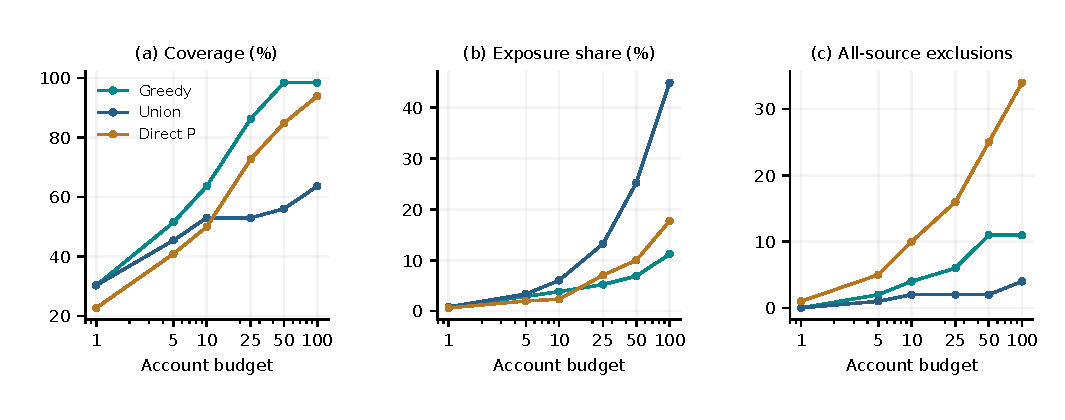
\includegraphics[width=0.98\textwidth]{revision_replication.pdf}
\caption{New-cohort name-graph comparisons across the six frozen budgets. Coverage uses 66 observed repository endpoints, H uses 2,494 account--repository pairs, and P excludes the source-free endpoint. Curves reuse one acquired cohort and supply no npm-wide uncertainty estimate.}
\label{fig:revision_replication}
\end{figure*}

Version continuity reduces pair mass from 2,494 to 2,411, a \ReplicationPairDecrease\% decrease. The corresponding decrease on the original graph was 42.44\%. The cohorts differ in roots, graph extent, versions and dates, so the comparison combines those changes. The coverage--exposure ordering repeats under both sets of observation conditions.

\subsection{Common Endpoints and Eligible Accounts}
Table~\ref{tab:revision_common} reports results on the common population.
% Generated by scripts/render_journal_validation.py
\begin{table*}[t]
\centering
\footnotesize
\caption{Reoptimized budget-100 selections on 65 common repository keys with 1,036 common selectable accounts.}
\label{tab:revision_common}
\begin{tabular}{llrrr}
\toprule
Dataset & Rule & $C$ & $H$ (\%) & $P$\\
\midrule
Original & Exact union & 52 & 21.55 & 4\\
Original & Greedy coverage & 65 & 6.09 & 8\\
Original & Original direct P & 65 & 11.72 & 20\\
New cohort & Exact union & 43 & 44.87 & 4\\
New cohort & Greedy coverage & 64 & 11.22 & 11\\
New cohort & Original direct P & 62 & 17.25 & 34\\
\bottomrule
\end{tabular}
\par\smallskip\begin{minipage}{0.98\textwidth}\footnotesize Complete source sets are preserved, including sources outside the common eligible account set. Pair denominators differ by observed graph, so H percentages are within-dataset quantities rather than a causal temporal effect.\end{minipage}
\end{table*}

We also reoptimize on 65 common repository keys with 1,036 accounts eligible in both datasets. Each dataset retains its full observed source sets, including origins outside the common candidate pool. H retains the relevant dataset's pair denominator. At budget 100, coverage remains greater for greedy than exact union in both graphs; the direct heuristic gives the largest P among these three compared rules. Top-100 Jaccard overlaps between reoptimized selections are 0.667 for exact union, 0.835 for greedy and 0.587 for direct exclusion. Shared observations and graph-bounding differences preclude treating these as independent ecosystem samples or a causal stability estimate.

\subsection{Consumer-side feasibility study}
A registry graph assigns downstream reach through observed dependency edges. To check how much of that reach can be traced in application-owned artifacts, we drew 40 repositories without replacement from 199 distinct GitHub repositories in the Awesome-Selfhosted index tagged JavaScript, TypeScript or Nodejs. We froze the index revision (\code{2a8926e0}), deterministic draw and midnight UTC cutoff on November 20, 2026 before inspecting consumer evidence. Each repository was pinned to a default-branch commit at or before the cutoff. None of the 40 appeared among the 7,171 original endpoint keys or the 66 endpoints used to train the October cohort rankings. The frame represents curated public self-hosted software.

Of 40 repositories, 34 supplied a root manifest and 17 a root npm lockfile. We evaluated eight with sufficiently supported inputs. Across the full draw, six lacked a root manifest, ten declared another manager, seven additional cases lacked a root npm lockfile, eight had unsupported inputs, and one contained an ambiguous or external path. These categories are mutually exclusive. For npm lockfile versions 2 and 3 we traced mandatory production dependencies from the root importer and checked declared ranges against locked versions. We compared each complete path with edges in npm Arborist's offline virtual tree. Both parsers use npm SemVer. This is a software cross-check of committed metadata. No packages were installed and no authors supplied manual labels.

Seven of eight compared projects yielded paths. The two parsers agreed on all 1,147 observed installation locations across those projects. Counting distinct package/version pairs separately per consumer yielded 1,110 observations. Of those, 278 could be linked through a public npm tarball identity to exact package/version maintainer metadata captured in the October cohort. Six projects supplied at least one such link. That metadata describes the earlier registry observation and cannot identify who controlled publication at a later date.

We evaluated the two greedy coverage portfolios frozen on the October cohort against these consumer paths. At budget 100, the name-based and version-based methods selected exactly the same 100 accounts. Both portfolios had a documented path in the same five projects. Three compared projects had no documented hit, and 32 drawn projects were unevaluable. Identical account lists necessarily cover the same projects when evaluated against the same files. The pilot shows how many projects we could evaluate and where the evidence ran out.

\subsection{Held-out consumer comparison}
\label{sec:consumer_holdout}
The pilot's identical 100-account greedy selections force equal project coverage. We therefore froze a five-account comparison on the October training graph before collecting the held-out application evidence. The name and version representations each use additive ranking. They share three of five accounts. We retain the original deterministic cutoff policy and score both alternative additive-optimal version portfolios separately. On the training repositories, the two deterministic portfolios each reach 30 repositories, including 25 shared and five exclusive to each. This training result motivates reporting changes in which consumers are covered alongside the change in total coverage.

The held-out frame comprises the remaining entries in the pinned Awesome-Selfhosted list after excluding all 40 pilot projects and repository keys that appear among earlier training endpoints. Each project is pinned to its public default HEAD when observed. We trace mandatory production dependencies from the root npm importer using committed lockfile formats 2 and 3. We corroborate the paths with npm Arborist's offline virtual tree. Workspaces, unsupported managers, unresolved paths and unavailable inputs contribute to the attrition ledger. The verification queue enumerates all distinct public package/version pairs corroborated by both implementations. We collect exact-version registry responses for this queue before matching any accounts to the portfolios. The registry fields describe observed maintainer-list associations during collection.

For each project and portfolio, a documented hit requires a corroborated path ending in an exact-version package with an observed selected account. A documented zero represents lack of a witness under the procedure. For full-reference coverage, we assign the set of paired statuses compatible with the evidence. A positive under both portfolios is fixed at $(1,1)$. A fully checked tree and registry join can justify an observed negative under the supported scope. When the unresolved evidence could change either outcome, we retain its feasible states. We compute the minimum and maximum of $|V-N|$ and $V-N$ within each project's feasible set and average those limits over the finite frame. The resulting bounds reflect incomplete evidence.

\begin{figure}[t]
\centering
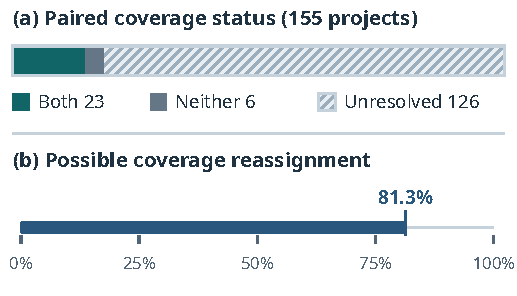
\includegraphics[width=\columnwidth]{consumer_holdout_evidence.pdf}
\caption{Paired consumer coverage evidence. The hatched segment shows unresolved pairs in the 155-application frame. The interval represents coverage reassignment compatible with the available evidence. All five-account tie choices give the same counts and bounds.}
\label{fig:consumer_holdout_evidence}
\end{figure}

We recorded all 155 projects and pinned 154 commits. Thirty projects entered the paired parser comparison and 25 yielded at least one corroborated path. The implementations agreed on 6,388 package locations in the compared projects. Arborist returned a virtual tree for 18 additional projects declined by the custom parser. Across the agreed paths, exact-version registry observations produced a usable maintainer list for 3,287 of 3,299 requested versions.

Figure~\ref{fig:consumer_holdout_evidence} shows the 23 documented common hits and six confirmed common negatives. Neither portfolio had an exclusive documented hit in any of the three comparisons. Each of the common hits had a witness from an account present in both portfolios. Twenty-nine outcomes were fully resolved, consisting of 23 common positives and six confirmed common negatives. The other 126 projects leave a full-reference turnover interval from 0 to 81.3\% and a net coverage interval from $-81.3$ to $+81.3$ percentage points. The identical-portfolio control gives zero turnover under all feasible assignments. The held-out study therefore cannot establish practical equivalence between the distinct portfolios. Access to applicable consumer trees is the primary measurement bottleneck in this frame.

\subsubsection{YunoHost comparison with broader lockfile support}
We applied the same frozen portfolios to a second frame of upstream applications from the YunoHost catalog. Requiring a root package manifest and excluding earlier repository keys and duplicate pinned commits yielded 215 projects. Lockfile intake identified 108 npm and 44 pnpm candidates. The other projects remain in the denominator.

For npm, we compare effective ranges from Arborist's virtual tree with checks against the committed dependency declarations, lockfile locations and pinned workspace manifests. The root walk follows verified links to local workspaces when those links are on a mandatory production path. Separate workspace importers are diagnostic because the catalog does not establish which importer is deployed. For pnpm lockfile format 9, we compare paths of up to three mandatory edges against the native offline listing. The depth limit lets those paths establish positive witnesses. A negative requires complete npm evidence within the supported root scope and an observed registry join for every retained witness.

We froze the comparison and the verification scope before acquiring the workspace manifests and observing the exact-version registry metadata used for scoring. A path's registry identity requires a canonical public npm tarball URL or an exact match between the lockfile's SHA-512 identifier and the registry response. We join maintainer associations after collection. Both frames measure committed dependency declarations and registry associations at the time of observation. The different intake and extraction rules limit direct comparisons between frames.

\section{Discussion}
\label{sec:discussion}
The practical choice begins with an objective. Coverage is suitable for distributing a review surface across distinct observed endpoints; additive H allocates selection toward account-origin pair mass under the stipulated weights; P requires selecting every observed source of a nonempty endpoint. The measured tradeoffs show that a defender cannot substitute one objective's score for another's. None of these quantities estimates how many incidents a real control prevents.

The additional experiments also distinguish useful evidence from mathematical expectation. Exact-union ranking's additive optimality follows from the objective; the empirical contribution is the associated coverage and exclusion cost. The new cohort repeats that direction while changing effect sizes. A representation effect of 42.44\% in one union and 3.33\% in the other warrants reporting population and version context whenever reach is compared.

The YunoHost frame shows why evaluation should track which applications each portfolio reaches. The five confirmed primary differences include both name-only and version-only outcomes. A net coverage statistic can hide these changes. The turnover lower bound is positive for every cutoff choice. Missing dependency evidence leaves the size and direction of the aggregate net change uncertain.

The recipe audit shows a separate measurement choice. The repository key, selected source revision, and package importer each matter for application reach. Even at the same commit, using the recipe's named frontend can change whether a dependency path is documented. Binary delivery requires tracing the provenance of the shipped artifact.

The exclusion heuristic illustrates why added complexity needs empirical justification. Reciprocal scoring is unnecessary for its original-graph P improvement, yet helps relative to the immediate variant in the new cohort. Candidate-restricted exact instances expose large empirical gaps despite frequent optimum matches. The present results support a transparent heuristic comparison, without a universal recommended cap or algorithmic guarantee.

The endpoint audit provides reproducible, commit-pinned evidence collection. Its automated indicators were not manually validated and do not establish mapping accuracy, workflow execution or historical validity. A deployment recommendation would additionally require observed authorization paths, intervention costs, feasible control policies and outcome evaluation. These missing measurements are separate from whether the retained graph computations are correct.

\section{Threats to Validity and Research Ethics}
\label{sec:threats_to_validity}
We organize limitations around construct, internal, external, and conclusion validity.

\subsection{Construct Validity}
Registry maintainer arrays supply username associations, not historical publication authority, token scope, account independence, or a peer-review policy. One maintainer does not prove absence of human review; several do not prove enforced review. Uniform and heterogeneous source weights are modeling assumptions. The perfect hardening model removes selected account origins, not package nodes or paths from other origins.

The workflow observation is a directory lookup at HEAD. The original acquisition lacks workflow YAML, job execution, permission scopes, historical release links, and consumer lockfiles. Fine-grained analyses of vulnerability propagation and localization use evidence from client code and dependent libraries~\cite{gao2025emse}. The workflow association measures a directory observed at collection time.
The new endpoint audit separately retains current commit-pinned workflows and selected manifests/lockfiles. It does not recover the missing original evidence. The automated indicators were not manually validated. Regular-expression and YAML-based extraction may miss reusable actions, infer the wrong working directory, or flag shell text that does not execute an install. These errors can affect the evidence-subset diagnostics.

The main exact-version graph is an observed deps.dev edge union, while the temporal companion is a bounded highest-satisfying SemVer approximation. They are different representations. Neither reconstructs npm hoisting, installed versions, overrides, or complete historical dependency trees. Runtime vulnerabilities are outside the package graph. Residual thresholds are hypothetical source-count rules, without signer groups, role constraints, or measured enforcement.

\subsection{Internal and Observational Validity}
Independent traversals, transposed source incidence, small-graph cases, and generated result checks validate computations on retained evidence. They cannot recover omitted observations. SCC condensation preserves reach; it is not a source of measured cycle-removal benefit. Ties use ascending username order, not portfolio size, except where portfolio size defines the selection rule itself.

Repository normalization is lexical. Excluding inconsistent positive observations tests sensitivity; it does not validate the other remote mappings or repair historical flags. Both main representations mix contexts and acquisition dates. Unknown workflow states and ambiguous zeros can omit eligible endpoints. Historical availability counts describe retained records, including a repeated tuple, and do not establish independent incidents or verified release authority.

\subsection{External and Conclusion Validity}
The high-impact-seeded expansion is neither registry-wide nor a random sample of npm installations. Public workflow-associated repositories cannot represent private consumer infrastructure without further evidence. Results describe this graph and explicit scenarios. They supply no measured compromise probabilities or causal control effects.
The new 100-root acquisition inherits the original ordinary-name sampling frame and observes a bounded cohort with only 66 eligible repository endpoints. Six failed dependency acquisitions and missing GitHub observations limit transport. Comparing full and common populations exposes scope differences but does not isolate time from population or graph extent. Two acquisitions do not supply independent temporal replicates. The small exact benchmarks deliberately use tractable candidate pools and retain outside sources; they cannot establish global approximation performance.

Random orders quantify selection variability. Orders are reused across nested budgets and endpoint definitions, so the resulting 6,000 rows are not independent ecosystem samples. Monte Carlo errors describe simulation means, not npm-wide uncertainty. The seven scalarization settings are exploratory tradeoff points, without a certified global Pareto frontier or an empirically estimated stakeholder preference. Heterogeneous weights are structural sensitivities, not fitted risk priors. Claims about efficacy require a separate intervention study.

The held-out comparisons draw from two curated application catalogs. The 155-project self-hosted frame retains projects with missing root manifests. The 215-project YunoHost frame requires a pinned root manifest and omits applications whose manifests are exclusively nested. Cross-tool agreement can miss shared errors. For pnpm, the depth limit restricts corroboration. The Yarn follow-up covers only the Classic subset and adds evidence from a separate registry collection. The bounds retain unresolved projects. Registry metadata records maintainer associations at observation time. Historical release authority requires separate evidence.

The recipe audits describe conditional samples. The fresh sample oversamples projects with observed workspace markers. Only two recipes permit matched path extraction under the archive, patch and parser checks. The single confirmed importer-sensitive case uses a post hoc closure check. Its verified sources support a dependency-declaration comparison. Packaging options and build steps can change what reaches a deployed application.

The release audit observes current public API responses and a bounded set of small archives. The checksum join tests consistency with the pinned recipe. Public endpoint responses delimit available evidence. Signed provenance and the completeness of an inventory require separate validation.

\subsection{Ethics and Reporting}
The analyses read retained public metadata and execute no package payloads, credential probes, or exploitation. Prospective captures omit email addresses and package bodies. Public usernames illustrate structural overlap without implying present-day insecurity, negligence, or historical publishing authority. Incident associations do not validate prediction. Artifact checksums identify retained bytes rather than certify authenticity.

\section{Conclusion}
\label{sec:conclusion}
Graph representation can change which applications enter documented review scope under the same account budget. At five accounts, the YunoHost comparison confirms three name-only and two version-only hits. The follow-ups resolve 164 of 215 pairs and bound turnover at 2.3--26.0\%. In Awesome-Selfhosted, they resolve 88 of 155 pairs, with no confirmed switches and turnover bounded at 0--43.2\%. The direction of net change remains unresolved in both frames. At 50 accounts, the exploratory YunoHost comparison identifies a separate switch.

The graph comparisons quantify a separate tradeoff. At 100 accounts on the original graph, greedy reaches 5,538 repositories and exact union reaches 4,407, with modeled exposure reductions of 11.48\% and 33.79\%, respectively. The coverage--exposure ordering repeats in the separately collected cohort, while the decrease in account--repository pair mass under version continuity changes from 42.44\% to 3.33\%. The exclusion heuristic has a worst deficit of 66 endpoints in the restricted exact benchmarks, and the relative performance of its variants changes across the two graphs.

A fixed-budget comparison can therefore report confirmed additions, removals, and unresolved cases alongside the total number of applications reached. The two consumer frames concern declared production paths at pinned commits and maintainer associations observed at collection time. Evaluating whether a control improves security requires separate evidence on authorization, deployment and intervention outcomes.

\section*{Statements and Declarations}

\subsection*{Funding}
This research received no external funding.

\subsection*{Competing Interests}
Both authors declare that they have no financial or non-financial competing interests relevant to this work.

\subsection*{Data Availability}
\providecommand{\ArtifactAccessStatement}{The October graph-validation data, analysis tables, protocols and checksums are available in the versioned research release \url{https://github.com/hasanshahriar32/npm-supply-chain-research/releases/tag/research-validation-2026-10-28}. The release includes a companion archive and links to the checksum-verified original database at a fixed repository commit. It provides derived audit observations and pinned URLs and hashes for third-party workflow, manifest and lockfile bodies.}
\ArtifactAccessStatement

The November consumer comparison has a separate replication archive
accompanying the submission. It includes the frozen dependency paths,
derived registry records, and pinned source references for the five
confirmed cases. It reproduces the paired outcomes, bounds, follow-ups,
and exploratory budget check from retained extraction outputs. The
projected registry records use numeric account indices. Full acquisition
replay requires the original source files and registry receipts.

\subsection*{Code Availability}
The October release includes the graph collection and analysis scripts, exact benchmark inputs, verification scripts, and figure-generation code. Its README describes checksum verification and reproduction from the original input. The November archive includes the scripts for the consumer analyses. Both numerical workflows use captured observations. A fresh acquisition may return different registry metadata.

\subsection*{Ethics and Consent}
The study analyzes public software-ecosystem metadata and does not involve recruited human participants, interventions on individuals, or execution of package payloads. No participant consent was collected. Usernames are used as observed graph identifiers, without inferring misconduct or present-day account security.


\section*{Acknowledgment}
We thank package maintainers, the open-source community, deps.dev and GitHub for public artifacts and interfaces.

\bibliographystyle{IEEEtran}
\bibliography{bibliography/references_q1}

\appendices
\section{Extended Objective Sensitivities}
\label{sec:objective_supplement}
\subsection{Exploratory Scalarization}
We evaluate $J_\alpha(S)=\alpha C(S)/|R_{\mathrm{wf}}|+(1-\alpha)H(S)$ at seven weights, $\alpha\in\{0,0.10,0.25,0.50,0.75,0.90,1\}$. These greedy solutions trace an observed tradeoff curve. Neither the finite weight sweep nor the approximation guarantee establishes the global Pareto frontier or a universally preferred weight.

Table~\ref{tab:q1_pareto_frontier} and Figure~\ref{fig:q1_pareto_frontier} summarize the evaluated scalarization settings.
% Auto-generated Pareto Frontier Table for Q1 Journal Expansion
\begin{table*}[t]
\centering
\small
\caption{Multi-objective Pareto frontier across scalarization weight $\alpha$ at budget $|S|=100$ ($|R_{\text{wf}}| = 7{,}171$).}
\label{tab:q1_pareto_frontier}
\begin{tabular}{lrrrrrrrr}
\toprule
& \multicolumn{4}{c}{Package-Projected Graph} & \multicolumn{4}{c}{Version-Continuous Graph}\\
\cmidrule(lr){2-5} \cmidrule(lr){6-9}
Scalarization $\alpha$ & $C$ & $C$ (\%) & $H$ (\%) & $P$ & $C$ & $C$ (\%) & $H$ (\%) & $P$\\
\midrule
0.00 (Exact Union) & 4,407 & 61.46\% & 33.79\% & 534 & 4,479 & 62.46\% & 40.59\% & 527\\
0.10 & 4,591 & 64.02\% & 33.65\% & 530 & 4,714 & 65.74\% & 40.37\% & 553\\
0.25 & 4,809 & 67.06\% & 32.98\% & 604 & 4,855 & 67.70\% & 39.94\% & 634\\
0.50 (Balanced Sweet Spot) & 5,020 & 70.00\% & 31.19\% & 626 & 5,000 & 69.73\% & 38.65\% & 648\\
0.75 & 5,403 & 75.35\% & 21.69\% & 779 & 5,239 & 73.06\% & 31.75\% & 695\\
0.90 & 5,529 & 77.10\% & 14.15\% & 794 & 5,509 & 76.82\% & 14.97\% & 826\\
1.00 (Greedy Coverage) & 5,538 & 77.23\% & 11.48\% & 800 & 5,516 & 76.92\% & 13.10\% & 817\\
\bottomrule
\end{tabular}
\end{table*}


\begin{figure}[t]
\centering
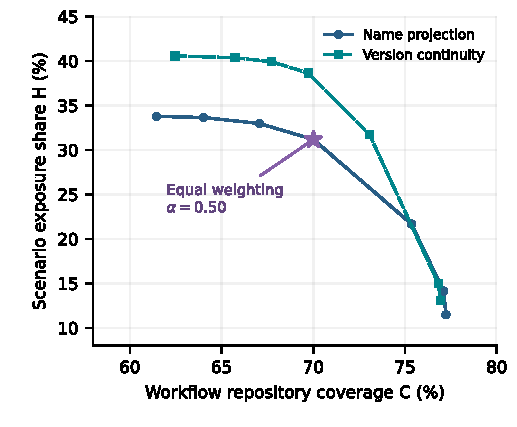
\includegraphics[width=\columnwidth]{q1_pareto_frontier.pdf}
\caption{Observed greedy scalarization results at budget 100. Connecting seven evaluated settings guides the eye; the curve is not a certified global Pareto frontier. Equal weighting is a sensitivity choice.}
\label{fig:q1_pareto_frontier}
\end{figure}

At $\alpha=0.50$, the name graph gives $C=5{,}020$, $H=31.19\%$, and $P=626$; the version graph gives $C=5{,}000$, $H=38.65\%$, and $P=648$. The name result retains 90.65\% of greedy's baseline coverage and 92.31\% of exact union's H. Relative to greedy, it loses 518 covered repositories and gains 19.71 percentage points of H. Relative to exact union, it gains 613 repositories and loses 2.60 points of H. A preferred operating point requires review costs and stakeholder preferences that were not measured here.

\subsection{Strict Zero-Anchored Threshold Sensitivity}
\label{sec:quorum_exclusion}

We evaluate the explicit strict rule in Eq.~\ref{eq:strict_quorum}, retaining only the 7,158 endpoints with observed sources and excluding all 13 source-free endpoints:
\begin{equation}
P_k(S)=\left|\left\{r\in R_+:t_r(S)=0\ \lor\ (n_r\ge k\ \land\ t_r(S)<k)\right\}\right|.
\end{equation}
The unguarded condition $t_r(S)<k$ credits every endpoint with $n_r<k$ even at zero hardening. In the strict model, a single-source endpoint must have its sole maintainer hardened at every threshold, and any endpoint with $n_r<k$ requires complete exclusion. This ensures a zero baseline for each tested $k$; it is not equivalent to subtracting the old zero-budget count.

A protection interpretation still requires a measured policy in which every successful attack needs the designated number of distinct upstream identities with no bypass. Our graph lacks package-level signer groups, role constraints, and bypass privileges. Two unrelated single-maintainer dependencies can each poison a consumer even if their combined source cardinality is two. Table~\ref{tab:q1_quorum_exclusion} is therefore a structural sensitivity analysis, not a count of empirically protected repositories.

% Auto-generated Generalized k-of-n Quorum Exclusion Table for Q1 Journal Expansion
\begin{table*}[t]
\centering
\small
\caption{Residual-source threshold counts $P_k(S)$ and coverage across maintainer hardening strategies ($|R_{\text{wf}}| = 7{,}171$).}
\label{tab:q1_quorum_exclusion}
\begin{tabular}{lrrrrrrrr}
\toprule
Prioritization Strategy & Budget & $C(S)$ & $C$ (\%) & $H(S)$ (\%) & $P_1(S)$ & $P_2(S)$ & $P_3(S)$ & $P_5(S)$ \\
 & $|S|$ & & & & ($k=1$) & ($k=2$) & ($k=3$) & ($k=5$) \\
\midrule
Portfolio Size                 & 10 & 3,435 & 47.90\% & 1.59\% & 391 & 1,915 & 2,433 & 3,093 \\
                               & 25 & 4,067 & 56.71\% & 4.38\% & 430 & 1,974 & 2,563 & 3,194 \\
                               & 50 & 4,446 & 62.00\% & 6.14\% & 503 & 2,025 & 2,613 & 3,244 \\
                               & 100 & 4,579 & 63.85\% & 7.96\% & 577 & 2,065 & 2,669 & 3,281 \\
\midrule
Greedy Coverage                & 10 & 4,331 & 60.40\% & 3.79\% & 351 & 1,846 & 2,406 & 3,080 \\
                               & 25 & 4,854 & 67.69\% & 6.08\% & 514 & 1,976 & 2,487 & 3,176 \\
                               & 50 & 5,196 & 72.46\% & 8.73\% & 638 & 2,039 & 2,552 & 3,232 \\
                               & 100 & 5,538 & 77.23\% & 11.48\% & 800 & 2,112 & 2,602 & 3,268 \\
\midrule
Exact Union                    & 10 & 3,910 & 54.53\% & 4.48\% & 343 & 1,825 & 2,385 & 3,105 \\
                               & 25 & 4,284 & 59.74\% & 9.86\% & 427 & 1,995 & 2,596 & 3,244 \\
                               & 50 & 4,321 & 60.26\% & 18.09\% & 441 & 2,011 & 2,609 & 3,324 \\
                               & 100 & 4,407 & 61.46\% & 33.79\% & 534 & 2,137 & 2,760 & 3,523 \\
\midrule
Pareto Hybrid ($\alpha=0.50$)  & 10 & 4,331 & 60.40\% & 3.79\% & 351 & 1,846 & 2,406 & 3,080 \\
                               & 25 & 4,795 & 66.87\% & 7.68\% & 498 & 1,948 & 2,505 & 3,194 \\
                               & 50 & 5,001 & 69.74\% & 14.96\% & 605 & 2,102 & 2,689 & 3,390 \\
                               & 100 & 5,020 & 70.00\% & 31.19\% & 626 & 2,153 & 2,719 & 3,415 \\
\midrule
Direct Supermodular $P(S)$     & 10 & 3,976 & 55.45\% & 2.58\% & 479 & 1,856 & 2,392 & 3,070 \\
                               & 25 & 4,239 & 59.11\% & 4.15\% & 618 & 1,880 & 2,424 & 3,124 \\
                               & 50 & 4,604 & 64.20\% & 6.55\% & 803 & 1,983 & 2,517 & 3,177 \\
                               & 100 & 5,020 & 70.00\% & 13.23\% & 1,022 & 2,074 & 2,636 & 3,337 \\
\bottomrule
\end{tabular}
\end{table*}


At budget 100, Pareto Hybrid has $P_1=626$, $P_2=961$, $P_3=1{,}018$, $P_5=1{,}063$. Greedy Coverage has $P_1=800$, $P_2=1{,}145$, $P_3=1{,}125$, $P_5=1{,}105$. Exact Union has $P_1=534$, $P_2=793$, $P_3=901$, $P_5=1{,}022$. Direct $P$ has $P_1=1{,}022$, $P_2=1{,}169$, $P_3=1{,}286$, $P_5=1{,}383$. The source-cardinality distribution is $n_r=0$: 13; $n_r=1$: 1,716; $n_r=2$: 546; $n_r=3$: 354; $n_r=4$: 347; and $n_r\ge5$: 4,195. All strict zero-budget counts are zero.

The same ordered maintainer selections are reused at all thresholds, and the Direct $P$ strategy continues to optimize its original $k=1$ heuristic. Counts are nondecreasing with nested hardening budgets for a fixed $k$. Comparisons across $k$ represent different hypothetical policies and need not be monotone, because endpoints with $n_r<k$ revert to complete-exclusion requirements.

For an additional hypothetical sensitivity, uniform control efficacy $\eta$ gives $H_\eta(S)=\eta H(S)$. At $\eta=0.90$, Pareto Hybrid yields $28.07\%$ effective scenario exposure reduction. This uniform multiplier preserves all $H$ rankings and does not estimate a real bypass rate, correlate account failures, or model CI compromise. Its values are assumptions, not incident-derived estimates.

\subsection{Heterogeneous Weight Sensitivities}
Table~\ref{tab:q1_heterogeneous_weights} compares the assumed weightings.
% Generated by scripts/reconcile_full_manuscript.py
\begin{table*}[t]
\centering
\footnotesize
\caption{Budget-100 outcomes under assumed weights. Each H column has its own stipulated denominator; weights are not estimated compromise probabilities.}
\label{tab:q1_heterogeneous_weights}
\begin{tabular}{lrrrrrr}
\toprule
Selection & C & H (\%) & Account-sole (\%) & Log (\%) & Package-sole (\%) & P\\
\midrule
Exact union & 4,407 & 33.79 & 77.30 & 40.15 & 27.32 & 534\\
Greedy coverage & 5,538 & 11.48 & 74.19 & 18.52 & 23.40 & 800\\
Portfolio & 4,579 & 7.96 & 70.26 & 15.06 & 13.72 & 577\\
Hybrid (0.50) & 5,020 & 31.19 & 80.41 & 38.93 & 28.51 & 626\\
Account-sole aware & 4,919 & 22.59 & 88.04 & 33.09 & 44.53 & 707\\
Log-portfolio aware & 4,603 & 31.91 & 81.42 & 42.91 & 33.17 & 514\\
Package-sole aware & 4,718 & 19.39 & 80.03 & 23.61 & 67.37 & 642\\
\bottomrule
\end{tabular}
\end{table*}


The account-sole weight increases an account's contribution according to its number of sole-maintained packages; it does not restrict its reachable endpoints to those packages. Ranking by that weighted reach captures 88.04\% of the stipulated account-sole mass. This is concentration under an assumed weighting, not nine-tenths of measured ecosystem risk.

The separate package-sole quantity unions reach only from each account's sole-maintained packages. Under that definition, unweighted greedy captures 23.40\%, unweighted exact union 27.32\%, and package-sole-aware ranking 67.37\%. The latter gain is 40.05 percentage points relative to unweighted exact union. Its uniform coverage is 4,718 repositories and $P=642$. These results distinguish account weighting from package-restricted reach. A single observed maintainer is not evidence about review quality or an empirically fitted probability of compromise.

\section{Consumer Evidence and Sensitivity Details}
\label{sec:consumer_evidence_details}
\subsection{Awesome-Selfhosted path corroboration}
The held-out frame comprises the remaining entries in the pinned Awesome-Selfhosted list after excluding all 40 pilot projects and repository keys that appear among earlier training endpoints. Each project is pinned to its public default HEAD when observed. We trace mandatory production dependencies from the root npm importer using committed lockfile formats 2 and 3. We corroborate the paths with npm Arborist's offline virtual tree. Workspaces, unsupported managers, unresolved paths and unavailable inputs contribute to the attrition ledger. The verification queue enumerates all distinct public package/version pairs corroborated by both implementations. We collect exact-version registry responses for this queue before matching any accounts to the portfolios. The registry fields describe observed maintainer-list associations during collection.

We recorded all 155 projects and pinned 154 commits. Thirty projects entered the paired parser comparison and 25 yielded at least one corroborated path. The implementations agreed on 6,388 package locations in the compared projects. Arborist returned a virtual tree for 18 additional projects declined by the custom parser. Across the agreed paths, exact-version registry observations produced a usable maintainer list for 3,287 of 3,299 requested versions.


\begin{figure}[t]
\centering
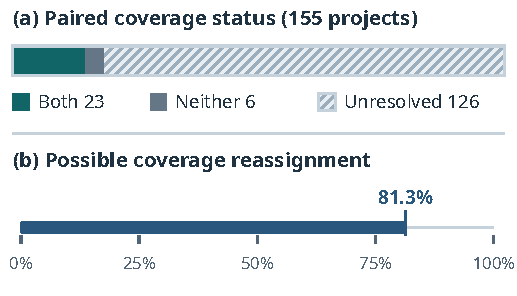
\includegraphics[width=\columnwidth]{consumer_holdout_evidence.pdf}
\caption{Paired consumer coverage evidence. The hatched segment shows unresolved pairs in the 155-application frame. The interval represents coverage reassignment compatible with the available evidence. All five-account tie choices give the same counts and bounds.}
\label{fig:consumer_holdout_evidence}
\end{figure}
\par Figure~\ref{fig:consumer_holdout_evidence} records the original evidence categories in this frame.

\subsection{YunoHost comparison with broader lockfile support}
The second frame comprises 215 upstream YunoHost projects with pinned root package manifests. We excluded earlier repository keys and duplicate pinned commits. Lockfile intake yielded 108 npm and 44 pnpm candidates. All 215 projects contribute to the paired comparison.

For npm, we compare effective ranges from Arborist's virtual tree with checks against the committed dependency declarations, lockfile locations and pinned workspace manifests. The root walk follows verified links to local workspaces when those links are on a mandatory production path. Separate workspace importers are diagnostic because the catalog does not establish which importer is deployed. For pnpm lockfile format 9, we compare paths of up to three mandatory edges against the native offline listing. The depth limit lets those paths establish positive witnesses. A negative requires complete npm evidence within the supported root scope and an observed registry join for every retained witness.

We froze the comparison and the verification scope before acquiring the workspace manifests and observing the exact-version registry metadata used for scoring. A path's registry identity requires a canonical public npm tarball URL or an exact match between the lockfile's SHA-512 identifier and the registry response. We join maintainer associations after collection. Both frames measure committed dependency declarations and registry associations at the time of observation. The different intake and extraction rules limit direct comparisons between frames.

On the same 108 npm candidates, the earlier reader returned corroborated locations for 50 projects and the expanded reader for 67. The readings share 8,158 package locations. The expanded procedure adds 5,463 locations in 19 projects, including three with root workspaces. It also leaves 316 previously corroborated locations unresolved in two projects. This comparison measures where the two procedures produce evidence on the same inputs.

The workspace collection returned all 15 requested manifests. The registry collection returned usable maintainer lists for 9,968 of 9,987 exact versions. Ninety projects have at least one registry-linked path. Seventy-two have complete path and registry evidence under the supported root scope. Positive witnesses under both portfolios also resolve pairs in projects with incomplete trees.

% Values from yunohost-v2, yunohost-yarn-classic and yunohost-empty-pnpm-roots results.json.
\begin{table}[t]
\centering
\footnotesize
\caption{Paired coverage in the 215-project YunoHost frame. Each column compares the name portfolio against a different additive-optimal version portfolio. Bounds account for unresolved pairs.}
\label{tab:yunohost_consumer_holdout}
\setlength{\tabcolsep}{3pt}
\begin{tabularx}{\linewidth}{@{}Yrrr@{}}
\toprule
Measure & Primary & Alt.~1 & Alt.~2\\
\midrule
\multicolumn{4}{@{}l}{\textit{Initial npm and pnpm analysis}}\\
Documented under both & 70 & 67 & 71\\
Documented name only & 4 & 7 & 3\\
Documented version only & 2 & 1 & 2\\
Documented under neither & 139 & 140 & 139\\
\addlinespace
Fully resolved pairs & 112 & 110 & 112\\
Fully resolved differences & 5 & 5 & 4\\
Turnover bounds (\%) & $[2.3,50.2]$ & $[2.3,51.2]$ & $[1.9,49.8]$\\
Net change bounds (pp) & $[-48.4,47.0]$ & $[-50.2,46.0]$ & $[-47.9,47.4]$\\
\addlinespace
\multicolumn{4}{@{}l}{\textit{After adding Yarn Classic evidence}}\\
Follow-up resolved pairs & 129 & 127 & 129\\
Follow-up turnover (\%) & $[2.3,42.3]$ & $[2.3,43.3]$ & $[1.9,41.9]$\\
Follow-up net change (pp) & $[-40.0,38.6]$ & $[-41.9,37.7]$ & $[-39.5,39.1]$\\
\addlinespace
\multicolumn{4}{@{}l}{\textit{Empty pnpm root sensitivity}}\\
Sensitivity resolved pairs & 145 & 143 & 145\\
Sensitivity turnover (\%) & $[2.3,34.9]$ & $[2.3,35.8]$ & $[1.9,34.4]$\\
Sensitivity net change (pp) & $[-32.6,31.2]$ & $[-34.4,30.2]$ & $[-32.1,31.6]$\\
\bottomrule
\end{tabularx}
\end{table}


In the primary comparison, 70 applications have documented hits under both portfolios and six have hits under just one. Five of those six are confirmed differences from fully checked roots (three name-only and two version-only). At least four pairs differ under each alternative cutoff tie, and three projects differ under all three choices. A post hoc check found a positive witness location corroborated by the earlier npm reader for every confirmed difference. The identical-portfolio control has zero turnover. The 103 unresolved primary pairs leave the total net coverage change compatible with either direction (Table~\ref{tab:yunohost_consumer_holdout}).

\subsection{Yarn Classic follow-up}
After the initial YunoHost analysis, we froze a follow-up protocol for its 35 Yarn candidates before collecting new registry evidence. Two lockfile readers checked the declared SemVer paths from each root. We excluded newer Yarn formats, workspace importers and edges affected by selective resolutions. Paths require canonical registry identifiers, SHA-512 agreement for Yarn mirror artifacts, and corroboration of transitive declarations against exact-version registry records. Yarn contributes positive witnesses only.

The readers agreed on 20 eligible lockfiles. Of 3,557 exact-version requests, 3,555 yielded usable maintainer lists. Nineteen applications have a registry-linked path. The added evidence resolves 17 further common hits in the primary comparison, raising the resolved count from 112 to 129. Two more applications have one documented portfolio hit and an unresolved counterpart. The turnover interval narrows to 2.3--42.3\% and the net interval to $-40.0$ to $+38.6$ percentage points. Both alternative cutoff choices show the same 17-pair increase (Table~\ref{tab:yunohost_consumer_holdout}). The follow-up retains the original observations for all other projects. Its bounds quantify the change from adding Yarn evidence collected separately.

\subsection{Sensitivity to empty pnpm roots}
The primary protocol uses pnpm paths to establish positive witnesses.
Among the 86 unresolved primary pairs after the Yarn follow-up, 23 had pnpm lockfile evidence. Sixteen of these had zero witnesses in a successful root comparison.
In a post hoc sensitivity analysis, we checked each of those 16 pinned
manifests and pnpm v9 root importers for regular dependency declarations.
All 16 had empty mandatory roots in both files. Thirteen declared
development dependencies. The other three had no development
declarations in the manifest. Under the mandatory root scope, these 16
applications are common negatives.

Adding these common negatives resolves 145 of 215 primary pairs and
leaves 70 unresolved. The turnover interval is 2.3--34.9\% and the net
interval is $-32.6$ to $+31.2$ percentage points. The five confirmed
differences persist. Table~\ref{tab:yunohost_consumer_holdout} also
reports the two alternative cutoff choices. The sensitivity covers
regular dependencies declared at the pinned root importer. Development
dependencies, other importers and release contents are outside this check.

\subsection{Newer Yarn, missing lockfiles and Bun}
We ran two further post hoc checks on unresolved projects. For all 14
newer Yarn candidates, we compared root declarations with the
\texttt{workspace:.} entry. Six roots had zero regular, optional,
peer or bundled dependencies. Their lock entries contain exactly the
development declarations from the pinned manifests. For all 18
projects without an available root lockfile, we checked the manifests
and lockfile receipts. Nine had empty production manifests, no declared
workspaces, and HTTP 404 receipts for all tested root lockfile names and
the pnpm workspace file. An empty declaration establishes a zero for
the root-scope estimand even when the capture has no lockfile. Taken
together, these checks add 15 common negatives and increase the number
of resolved primary pairs to 160 (Table~\ref{tab:yunohost_consumer_holdout}).

We also screened all six unresolved Bun projects for direct evidence.
Two had supported text lockfiles and matching root declarations
without overrides or patches. Across these two projects, 14 exact
versions matched the SHA-512 values in retained npm registry receipts.
The locked \texttt{p-queue} 10.0.0 at project Y473 supplies a
shared hit for the name selection and all three version alternatives.
This positive-only check resolves one more project. The combined
sensitivity resolves 161 of 215 primary pairs. Feasible turnover is
2.3--27.4\%, and net change is $-25.1$ to $+23.7$ percentage points.
The five confirmed coverage changes persist. The results concern
declared paths from a pinned root. Other workspace roots and
dependencies introduced during packaging are outside this comparison.

\subsection{Checks on unresolved npm roots}
We examined all 17 unresolved npm projects for empty production
roots or additional verifiable identities. Three root manifests had no
regular, optional, peer or bundled dependencies and corroborating
lockfile evidence. Two had matching root declarations in v3 lockfiles.
The third had a v1 lockfile with all 806 entries marked
development-only and locked root development versions satisfying the
manifest ranges. We left two other empty manifests unresolved because
their version labels disagree with the lockfiles.

Two projects had complete path extraction but incomplete registry
identity. We found 62 locations across them with neither a tarball URL
nor usable SHA-512. Checking direct v1 dependencies against retained
registry receipts supplied no additional hits. Adding the three
corroborated zeros resolves 164 primary pairs and leaves 51 unresolved.
The turnover bounds narrow to 2.3--26.0\%, and net change remains
compatible with either direction ($-23.7$ to $+22.3$ percentage points).
This is a post hoc sensitivity within the same declared root scope.


\section{Consumer Packaging and Release Diagnostics}
\label{sec:consumer_packaging}
\subsection{Packaging recipe and importer check}
The upstream repository root can differ from the directory selected for packaging. We examined the catalog-pinned YunoHost recipes for 15 unresolved projects with empty pnpm workspace roots and 16 without a conventional root lockfile. We checked source declarations, install and upgrade instructions, and available service templates. Twelve of the 15 workspace recipes install a release artifact or distribution package. Of the remaining three, one delegates asset compilation without selecting a named importer in the observed recipe, one builds a named frontend workspace, and one builds a workspace and copies a named client into a named server. Three of the 16 missing-root-lockfile recipes contain explicit npm dependency commands. One uses a nested server lockfile. The other two lack a committed npm lockfile at the recipe-selected root.

We resolved the source references for all six recipes with explicit JavaScript package commands. Four select commits different from the upstream commits observed in the root study. The three recipes with named importers and lockfiles yield four importer paths across three applications. We verified each declared source archive checksum and checked that the selected manifest and lockfile bytes match the pinned Git files. These three packaging trees contain no source patches in the checked locations. The comparison traces mandatory dependency declarations from the selected importers, using the same three portfolios and tie policy. It describes the packaging recipe's inputs. Runtime inclusion and installed versions would require separate evidence.

We corroborated 425 paths across the four importers and obtained usable maintainer lists for all 401 requested versions. All three applications had documented hits under both portfolios for every version cutoff choice. In the same-commit case, the recipe-selected frontend supplies paths that the empty upstream root cannot provide. The other two recipes use different commits from the root study. This diagnostic uses a separate three-application denominator. The 215-project comparison retains its root-importer scope and bounds.

\subsection{Same-commit comparison on a fresh recipe sample}
We froze 99 previously unaudited recipes from the catalog frame. The sample includes all 39 remaining repositories with an observed workspace marker and a seeded draw of 60 from the other 430. Seven recipes name a non-root importer involved in a build or service (six in the workspace stratum and one in the other stratum). Six of the seven select Git commits different from the screened upstream HEADs. Four source archives and their corresponding Git files could be checked by hash. One of the four has packaging patches and another uses an unsupported Yarn workspace. The remaining two permit a comparison at a fixed recipe-selected commit, using the same 772 exact-version requests across both views of the application. We obtained 771 usable maintainer lists.

In one application, the root yielded 83 joined paths and the selected backend lockfile lacked registry artifact identifiers for its corroborated paths. The second yielded one joined root path and 725 joined paths across its selected workspaces. Under the prespecified completeness rule, both root-to-importer coverage changes remained unresolved. A post hoc check found that the second root had exactly one mandatory dependency, no mandatory children in the lock or exact-version metadata, and consistent artifact and maintainership records. With this confirmed root zero, selecting the recipe's importers produces a documented gain for the name portfolio and all three version alternatives. This establishes one importer-sensitive case under the declared dependency scope. Six named candidates remain unresolved, and the 99-recipe sample supplies no population-wide effect estimate.

\subsection{Release-delivered dependency evidence}
We followed the 39 recipes in the fresh sample that declared a release asset and had no matched JavaScript package command. Literal setup instructions identify 38 GitHub assets across 37 recipes, using amd64 resource fields where specified. The release API identifies 37 assets. Thirty reported SHA-256 values agree with the recipe pins, six lack an API digest, and one differs. Public attestation lookups for the 30 agreeing digests return subject-matching statements for six assets. Three SLSA provenance statements declare source commits for their release repositories. We parse the statements without verifying signatures. A separate CycloneDX document identifies the selected Java runtime by filename and exact digest. That inventory contains no npm package URLs.

We downloaded the 15 identified assets within a 12\,MiB cap. Fourteen matched their recipe checksum, including five with no API digest. The mismatching download agreed with the API digest. Eleven matching ZIP or gzip TAR archives could be inspected. One contained 198 bundled npm manifests whose metadata lacked the registry artifact identifiers required for the metadata join. Another contained an application manifest and a Yarn Classic lockfile. These two releases support separate checks on declared dependencies and on packaged files.

\subsection{Declared dependencies in a pinned release}
The Pterodactyl panel archive is the one inspected artifact with both a Node manifest and a Yarn Classic lockfile. Its checksum agrees with the recipe, and both dependency files match the commit resolved from its source release tag byte for byte. We processed both views with the same reader and registry snapshot. Of 252 exact-version requests, all returned usable maintainer lists. The path checks corroborate 224 package versions in each view and document hits under the name portfolio and all three version alternatives. The equal results reflect the identical metadata inputs. The archive also includes 17 JavaScript files under its public assets directory. The lockfile evidence does not trace which of its declared dependencies are present in those files.

\subsection{Evidence in shipped JavaScript and dependency files}
We statically parsed all 17 public JavaScript assets in the Pterodactyl archive. The assets directory contains no source-map files, and the JavaScript contains no source-map directive comments. The sole \texttt{sourceMappingURL} occurrence is inside a string literal. The tagged Webpack configuration disables source maps by default in production, with an environment setting that can override the default. The archive and configuration thus delimit the available evidence for tracing bundled modules in this release.

The Mongo Express archive preserves a \texttt{node\_modules} tree. The packaged versions of all 39 regular direct dependencies satisfy the application's declared ranges. For each of these versions, we checked the npm tarball against the registry's SHA-512 integrity value. We then compared the relative paths and SHA-256 hashes of regular files within each dependency directory, excluding nested \texttt{node\_modules} in both archives. All 39 dependencies matched across 1,571 file paths. Using maintainer lists observed for those versions, the name portfolio and all three version alternatives reached the application through a dependency whose files were present in the release. This diagnostic measures file inclusion for direct dependencies in one archive. Runtime loading and transitive completeness remain outside its scope.



\end{document}
